% Options for packages loaded elsewhere
\PassOptionsToPackage{unicode}{hyperref}
\PassOptionsToPackage{hyphens}{url}
\PassOptionsToPackage{dvipsnames,svgnames,x11names}{xcolor}
%
\documentclass[
  letterpaper,
  DIV=11,
  numbers=noendperiod]{scrreprt}

\usepackage{amsmath,amssymb}
\usepackage{lmodern}
\usepackage{iftex}
\ifPDFTeX
  \usepackage[T1]{fontenc}
  \usepackage[utf8]{inputenc}
  \usepackage{textcomp} % provide euro and other symbols
\else % if luatex or xetex
  \usepackage{unicode-math}
  \defaultfontfeatures{Scale=MatchLowercase}
  \defaultfontfeatures[\rmfamily]{Ligatures=TeX,Scale=1}
\fi
% Use upquote if available, for straight quotes in verbatim environments
\IfFileExists{upquote.sty}{\usepackage{upquote}}{}
\IfFileExists{microtype.sty}{% use microtype if available
  \usepackage[]{microtype}
  \UseMicrotypeSet[protrusion]{basicmath} % disable protrusion for tt fonts
}{}
\makeatletter
\@ifundefined{KOMAClassName}{% if non-KOMA class
  \IfFileExists{parskip.sty}{%
    \usepackage{parskip}
  }{% else
    \setlength{\parindent}{0pt}
    \setlength{\parskip}{6pt plus 2pt minus 1pt}}
}{% if KOMA class
  \KOMAoptions{parskip=half}}
\makeatother
\usepackage{xcolor}
\setlength{\emergencystretch}{3em} % prevent overfull lines
\setcounter{secnumdepth}{5}
% Make \paragraph and \subparagraph free-standing
\ifx\paragraph\undefined\else
  \let\oldparagraph\paragraph
  \renewcommand{\paragraph}[1]{\oldparagraph{#1}\mbox{}}
\fi
\ifx\subparagraph\undefined\else
  \let\oldsubparagraph\subparagraph
  \renewcommand{\subparagraph}[1]{\oldsubparagraph{#1}\mbox{}}
\fi

\usepackage{color}
\usepackage{fancyvrb}
\newcommand{\VerbBar}{|}
\newcommand{\VERB}{\Verb[commandchars=\\\{\}]}
\DefineVerbatimEnvironment{Highlighting}{Verbatim}{commandchars=\\\{\}}
% Add ',fontsize=\small' for more characters per line
\usepackage{framed}
\definecolor{shadecolor}{RGB}{241,243,245}
\newenvironment{Shaded}{\begin{snugshade}}{\end{snugshade}}
\newcommand{\AlertTok}[1]{\textcolor[rgb]{0.68,0.00,0.00}{#1}}
\newcommand{\AnnotationTok}[1]{\textcolor[rgb]{0.37,0.37,0.37}{#1}}
\newcommand{\AttributeTok}[1]{\textcolor[rgb]{0.40,0.45,0.13}{#1}}
\newcommand{\BaseNTok}[1]{\textcolor[rgb]{0.68,0.00,0.00}{#1}}
\newcommand{\BuiltInTok}[1]{\textcolor[rgb]{0.00,0.23,0.31}{#1}}
\newcommand{\CharTok}[1]{\textcolor[rgb]{0.13,0.47,0.30}{#1}}
\newcommand{\CommentTok}[1]{\textcolor[rgb]{0.37,0.37,0.37}{#1}}
\newcommand{\CommentVarTok}[1]{\textcolor[rgb]{0.37,0.37,0.37}{\textit{#1}}}
\newcommand{\ConstantTok}[1]{\textcolor[rgb]{0.56,0.35,0.01}{#1}}
\newcommand{\ControlFlowTok}[1]{\textcolor[rgb]{0.00,0.23,0.31}{#1}}
\newcommand{\DataTypeTok}[1]{\textcolor[rgb]{0.68,0.00,0.00}{#1}}
\newcommand{\DecValTok}[1]{\textcolor[rgb]{0.68,0.00,0.00}{#1}}
\newcommand{\DocumentationTok}[1]{\textcolor[rgb]{0.37,0.37,0.37}{\textit{#1}}}
\newcommand{\ErrorTok}[1]{\textcolor[rgb]{0.68,0.00,0.00}{#1}}
\newcommand{\ExtensionTok}[1]{\textcolor[rgb]{0.00,0.23,0.31}{#1}}
\newcommand{\FloatTok}[1]{\textcolor[rgb]{0.68,0.00,0.00}{#1}}
\newcommand{\FunctionTok}[1]{\textcolor[rgb]{0.28,0.35,0.67}{#1}}
\newcommand{\ImportTok}[1]{\textcolor[rgb]{0.00,0.46,0.62}{#1}}
\newcommand{\InformationTok}[1]{\textcolor[rgb]{0.37,0.37,0.37}{#1}}
\newcommand{\KeywordTok}[1]{\textcolor[rgb]{0.00,0.23,0.31}{#1}}
\newcommand{\NormalTok}[1]{\textcolor[rgb]{0.00,0.23,0.31}{#1}}
\newcommand{\OperatorTok}[1]{\textcolor[rgb]{0.37,0.37,0.37}{#1}}
\newcommand{\OtherTok}[1]{\textcolor[rgb]{0.00,0.23,0.31}{#1}}
\newcommand{\PreprocessorTok}[1]{\textcolor[rgb]{0.68,0.00,0.00}{#1}}
\newcommand{\RegionMarkerTok}[1]{\textcolor[rgb]{0.00,0.23,0.31}{#1}}
\newcommand{\SpecialCharTok}[1]{\textcolor[rgb]{0.37,0.37,0.37}{#1}}
\newcommand{\SpecialStringTok}[1]{\textcolor[rgb]{0.13,0.47,0.30}{#1}}
\newcommand{\StringTok}[1]{\textcolor[rgb]{0.13,0.47,0.30}{#1}}
\newcommand{\VariableTok}[1]{\textcolor[rgb]{0.07,0.07,0.07}{#1}}
\newcommand{\VerbatimStringTok}[1]{\textcolor[rgb]{0.13,0.47,0.30}{#1}}
\newcommand{\WarningTok}[1]{\textcolor[rgb]{0.37,0.37,0.37}{\textit{#1}}}

\providecommand{\tightlist}{%
  \setlength{\itemsep}{0pt}\setlength{\parskip}{0pt}}\usepackage{longtable,booktabs,array}
\usepackage{calc} % for calculating minipage widths
% Correct order of tables after \paragraph or \subparagraph
\usepackage{etoolbox}
\makeatletter
\patchcmd\longtable{\par}{\if@noskipsec\mbox{}\fi\par}{}{}
\makeatother
% Allow footnotes in longtable head/foot
\IfFileExists{footnotehyper.sty}{\usepackage{footnotehyper}}{\usepackage{footnote}}
\makesavenoteenv{longtable}
\usepackage{graphicx}
\makeatletter
\def\maxwidth{\ifdim\Gin@nat@width>\linewidth\linewidth\else\Gin@nat@width\fi}
\def\maxheight{\ifdim\Gin@nat@height>\textheight\textheight\else\Gin@nat@height\fi}
\makeatother
% Scale images if necessary, so that they will not overflow the page
% margins by default, and it is still possible to overwrite the defaults
% using explicit options in \includegraphics[width, height, ...]{}
\setkeys{Gin}{width=\maxwidth,height=\maxheight,keepaspectratio}
% Set default figure placement to htbp
\makeatletter
\def\fps@figure{htbp}
\makeatother
\newlength{\cslhangindent}
\setlength{\cslhangindent}{1.5em}
\newlength{\csllabelwidth}
\setlength{\csllabelwidth}{3em}
\newlength{\cslentryspacingunit} % times entry-spacing
\setlength{\cslentryspacingunit}{\parskip}
\newenvironment{CSLReferences}[2] % #1 hanging-ident, #2 entry spacing
 {% don't indent paragraphs
  \setlength{\parindent}{0pt}
  % turn on hanging indent if param 1 is 1
  \ifodd #1
  \let\oldpar\par
  \def\par{\hangindent=\cslhangindent\oldpar}
  \fi
  % set entry spacing
  \setlength{\parskip}{#2\cslentryspacingunit}
 }%
 {}
\usepackage{calc}
\newcommand{\CSLBlock}[1]{#1\hfill\break}
\newcommand{\CSLLeftMargin}[1]{\parbox[t]{\csllabelwidth}{#1}}
\newcommand{\CSLRightInline}[1]{\parbox[t]{\linewidth - \csllabelwidth}{#1}\break}
\newcommand{\CSLIndent}[1]{\hspace{\cslhangindent}#1}

\KOMAoption{captions}{tableheading}
\makeatletter
\makeatother
\makeatletter
\@ifpackageloaded{bookmark}{}{\usepackage{bookmark}}
\makeatother
\makeatletter
\@ifpackageloaded{caption}{}{\usepackage{caption}}
\AtBeginDocument{%
\ifdefined\contentsname
  \renewcommand*\contentsname{Table of contents}
\else
  \newcommand\contentsname{Table of contents}
\fi
\ifdefined\listfigurename
  \renewcommand*\listfigurename{List of Figures}
\else
  \newcommand\listfigurename{List of Figures}
\fi
\ifdefined\listtablename
  \renewcommand*\listtablename{List of Tables}
\else
  \newcommand\listtablename{List of Tables}
\fi
\ifdefined\figurename
  \renewcommand*\figurename{Figure}
\else
  \newcommand\figurename{Figure}
\fi
\ifdefined\tablename
  \renewcommand*\tablename{Table}
\else
  \newcommand\tablename{Table}
\fi
}
\@ifpackageloaded{float}{}{\usepackage{float}}
\floatstyle{ruled}
\@ifundefined{c@chapter}{\newfloat{codelisting}{h}{lop}}{\newfloat{codelisting}{h}{lop}[chapter]}
\floatname{codelisting}{Listing}
\newcommand*\listoflistings{\listof{codelisting}{List of Listings}}
\makeatother
\makeatletter
\@ifpackageloaded{caption}{}{\usepackage{caption}}
\@ifpackageloaded{subcaption}{}{\usepackage{subcaption}}
\makeatother
\makeatletter
\@ifpackageloaded{tcolorbox}{}{\usepackage[many]{tcolorbox}}
\makeatother
\makeatletter
\@ifundefined{shadecolor}{\definecolor{shadecolor}{rgb}{.97, .97, .97}}
\makeatother
\makeatletter
\makeatother
\ifLuaTeX
  \usepackage{selnolig}  % disable illegal ligatures
\fi
\IfFileExists{bookmark.sty}{\usepackage{bookmark}}{\usepackage{hyperref}}
\IfFileExists{xurl.sty}{\usepackage{xurl}}{} % add URL line breaks if available
\urlstyle{same} % disable monospaced font for URLs
\hypersetup{
  pdftitle={R for Physicians: Learning with Ease \& Efficiency},
  pdfauthor={Ernie Pedapati, MD},
  colorlinks=true,
  linkcolor={blue},
  filecolor={Maroon},
  citecolor={Blue},
  urlcolor={Blue},
  pdfcreator={LaTeX via pandoc}}

\title{R for Physicians: Learning with Ease \& Efficiency}
\author{Ernie Pedapati, MD}
\date{6/12/23}

\begin{document}
\maketitle
\ifdefined\Shaded\renewenvironment{Shaded}{\begin{tcolorbox}[enhanced, sharp corners, breakable, frame hidden, borderline west={3pt}{0pt}{shadecolor}, boxrule=0pt, interior hidden]}{\end{tcolorbox}}\fi

\renewcommand*\contentsname{Table of contents}
{
\hypersetup{linkcolor=}
\setcounter{tocdepth}{2}
\tableofcontents
}
\bookmarksetup{startatroot}

\hypertarget{preface}{%
\chapter*{Preface}\label{preface}}
\addcontentsline{toc}{chapter}{Preface}

\markboth{Preface}{Preface}

Welcome to your essential guide to learning R for medical professionals.
If you're a physician eager to master R, you may find yourself at a
crossroads. On the one hand, you have the vast online universe of random
tutorials, StackOverflow threads, and YouTube videos. On the other, you
have highly-reviewed online courses that promise a comprehensive
understanding of R but often don't cater to your specific needs as a
medical professional.

This book is different.

As a physician who ventured into the world of R post-residency (and now
uses it daily), I found myself mired in information overload. Online
resources, while immensely helpful, were scattered and disjointed.
Online courses, on the other hand, offered structure but lacked the
specific context that physicians need. This gap is what led me to pen
this guide - a streamlined, context-rich resource tailor-made for
physicians.

This guide is built on real-life experiences and hurdles that I faced in
my journey of learning R. The issues that confused me, the challenges
that stumped me, the ``aha'' moments I had - they're all in here. But
more than that, this guide anticipates and addresses the likely issues
that you, as a physician learning R, will encounter.

Each chapter is a step further in your journey, with examples and
use-cases centered around medical scenarios, making the learning
experience highly relevant and practical for you. Whether it's data
manipulation, statistical analysis, or data visualization, the examples
and use-cases are drawn from medical scenarios to make your learning
experience as relevant as possible.

Embrace this guide as an ally in your pursuit of R mastery. It's a
journey that's already been tread, with roadblocks cleared and signposts
erected for easy navigation. This book isn't about wandering aimlessly
through tutorials, it's about embarking on a well-blazed trail,
specifically charted for physicians by a physician. So welcome aboard,
let's turn the page and commence our shared adventure.

\bookmarksetup{startatroot}

\hypertarget{introduction}{%
\chapter{Introduction}\label{introduction}}

\hypertarget{what-is-r}{%
\section{What is R?}\label{what-is-r}}

R is a free, open-source programming language and software environment
specifically designed for statistical computing and graphics. Ross Ihaka
and Robert Gentleman created R at the University of Auckland and it is
now maintained by the R Development Core Team. R is essentially composed
of a core language and a variety of user interfaces. The core language,
often referred to as ``base R'', is where all the computation and
processing happens. The user interfaces, such as RStudio, provide an
intuitive frontend where users write code, visualize data, and manage
their workflows.

The idea for R came about when Drs. Ross Ihaka and Robert Gentleman were
teaching an introductory statistics course and were unsatisfied with the
statistical software available to them. They wanted to create a software
that was free, user-friendly, and provided an effective way to teach
their students statistics.

Interestingly, R is named partly after the first names of the two R
authors (Robert and Ross) and partly as a play on the name of S, an
influential statistical programming language at the time.

Since its creation, R has grown exponentially, with a vibrant community
of users and developers from various fields like academia, industry, and
data science. It's maintained by a large, global group of volunteers who
continually add to its capabilities by creating new packages.

\hypertarget{why-r}{%
\section{Why R?}\label{why-r}}

For those of us who've engaged with statistical analysis during our
education or careers, the memory of installing a hard-to-get software
replete with countless menus, allowing interaction primarily through
mouse clicks, is all too familiar. Perhaps you ran various commands on
data, or dove into different analyses, all while navigating through
these menus and outputs. I recall those times vividly and suspect many
of you have similar experiences.

R, to many, might initially appear as an obscure programming language
tucked away in academia or tech-based industries.

But let me challenge your perception!

The very traits of R that lend it an air of obscurity are, in fact, its
most significant assets.

\hypertarget{great-things-about-r}{%
\section{Great things about R}\label{great-things-about-r}}

\begin{enumerate}
\def\labelenumi{\arabic{enumi}.}
\item
  \textbf{You don't have to install R}:

  Unlike traditional software, R doesn't demand space on your computer.
  It runs smoothly in the cloud, making it accessible from anywhere, on
  any device. More importantly, the scripts, the `statistical documents'
  you write in R, are not one-off commands. They are reusable, editable,
  and shareable pieces of code that capture your entire analytical
  process from start to finish.
\item
  \textbf{R is free:}

  I still have bad memories of trying to find a student copy of an
  expensive statistics software I bought in college. The complete and
  latest R suite is free to run on the platform of your choice and the
  100\% cloud-based R-Studio has a generous amount of resources for
  their free plan.
\item
  \textbf{Active and Friendly Community:}

  R has a large, active, and helpful user community. This means help is
  often readily available through online forums, blogs, and tutorials.
\item
  \textbf{Narratives, not isolation:}

  Writing scripts in R provides a natural and coherent flow to your
  work, a linear narrative, if you will. Instead of isolated tables and
  analyses separated by an output window, you have a comprehensive,
  logical story.
\item
  \textbf{Awesome outputs:}

  The table and graphics capabilities of R are second to none. Packages
  such as \texttt{flextable} and \texttt{ggplot2} provide advanced
  functionality for creating high-quality, customizable, and
  publication-ready graphics. You will quickly recognize in print and
  media that R is everywhere!
\end{enumerate}

After spending some time with R, becoming familiar with its
capabilities, and experiencing its versatility firsthand, you might find
it hard to even recognize it compared to the statistical programs you
used back in college.

\hypertarget{using-rstudio-cloud}{%
\section{Using RStudio Cloud}\label{using-rstudio-cloud}}

RStudio Cloud is a great tool that simplifies the process of setting up
R. It allows you to run R directly from your web browser, eliminating
the need to install software locally and handle any setup hassles. In
2023, RStudio was renamed Posit Studio and Posit Cloud but in this book,
I will continue to refer to it as RStudio and RCloud.

\begin{enumerate}
\def\labelenumi{\arabic{enumi}.}
\item
  \textbf{Creating an Account}

  First, navigate to the RStudio Cloud website
  (\href{https://rstudio.cloud/}{\textbf{https://rstudio.cloud/}}). If
  you don't have an account yet, click on ``Sign Up'' to create one.
  Enter your details, then click ``Register''. You'll receive an email
  to confirm your account.

  \begin{quote}
  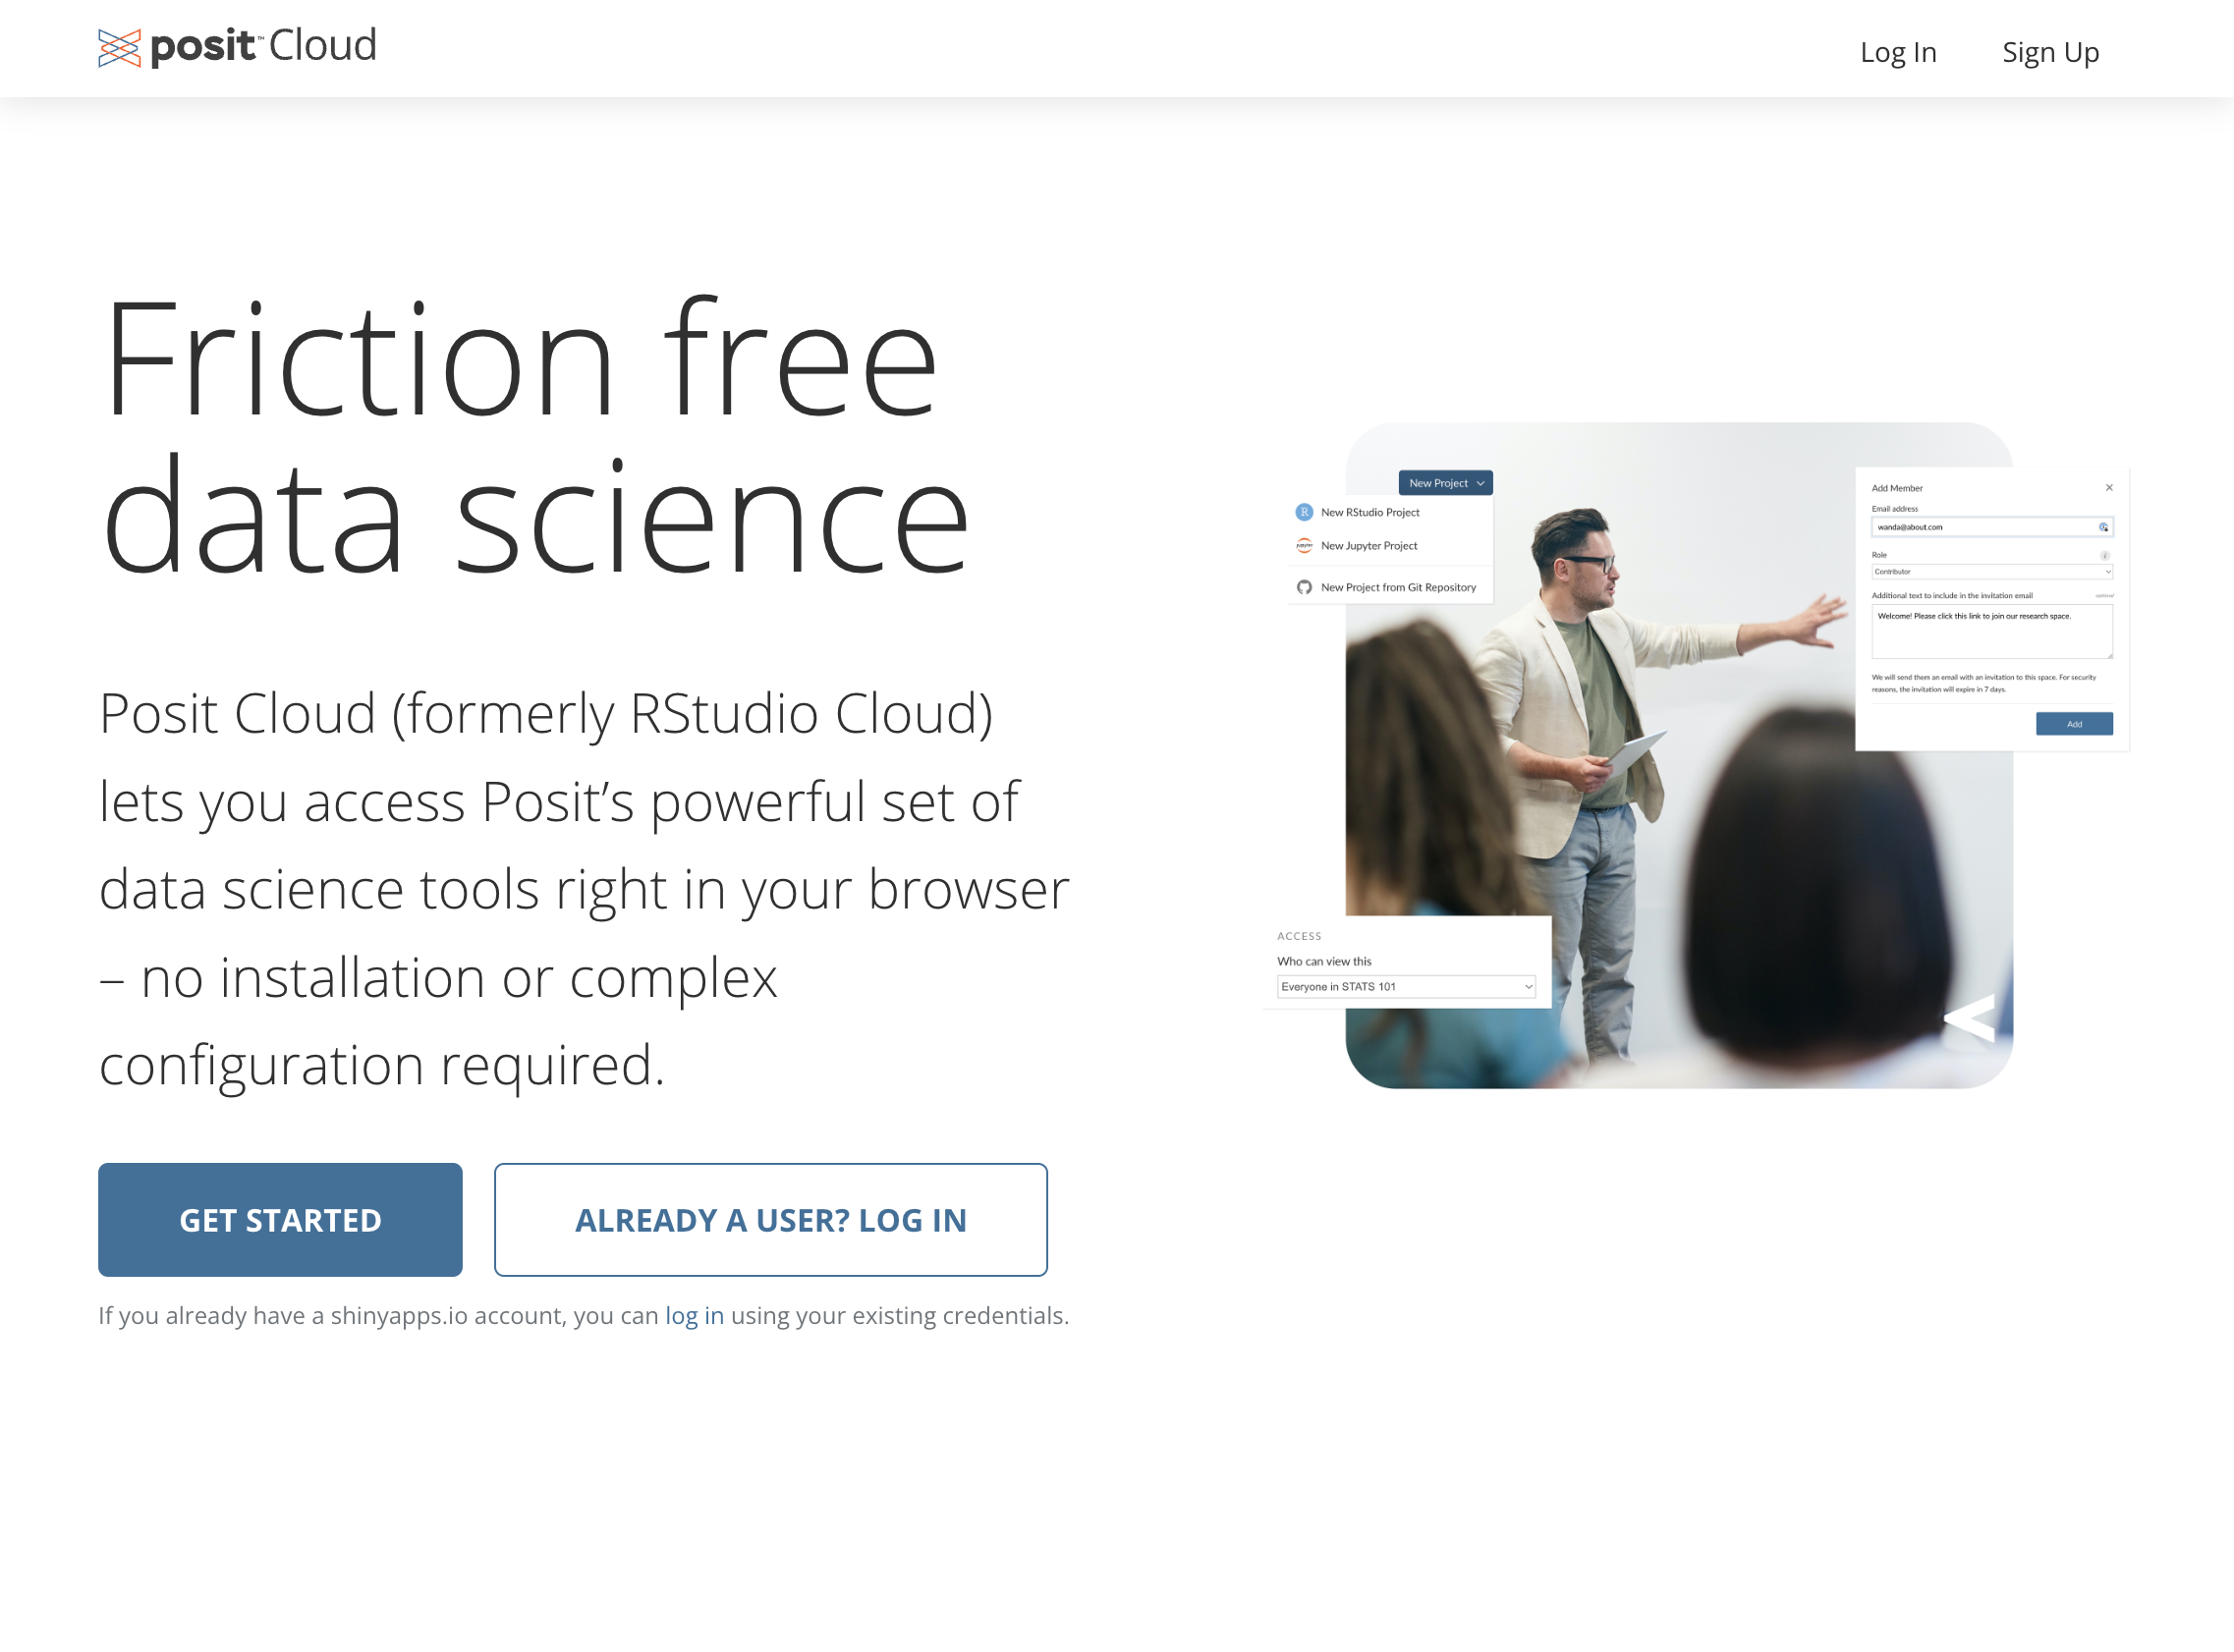
\includegraphics{./images/posit.cloud_ (1).png}
  \end{quote}
\item
  \textbf{Creating a New Project}

  After you've logged in, you'll see your RStudio Cloud workspace. Click
  on the ``New Project'' button to start a new R project. Enter a name
  for your project and then click on ``Create Project''.

  \begin{quote}
  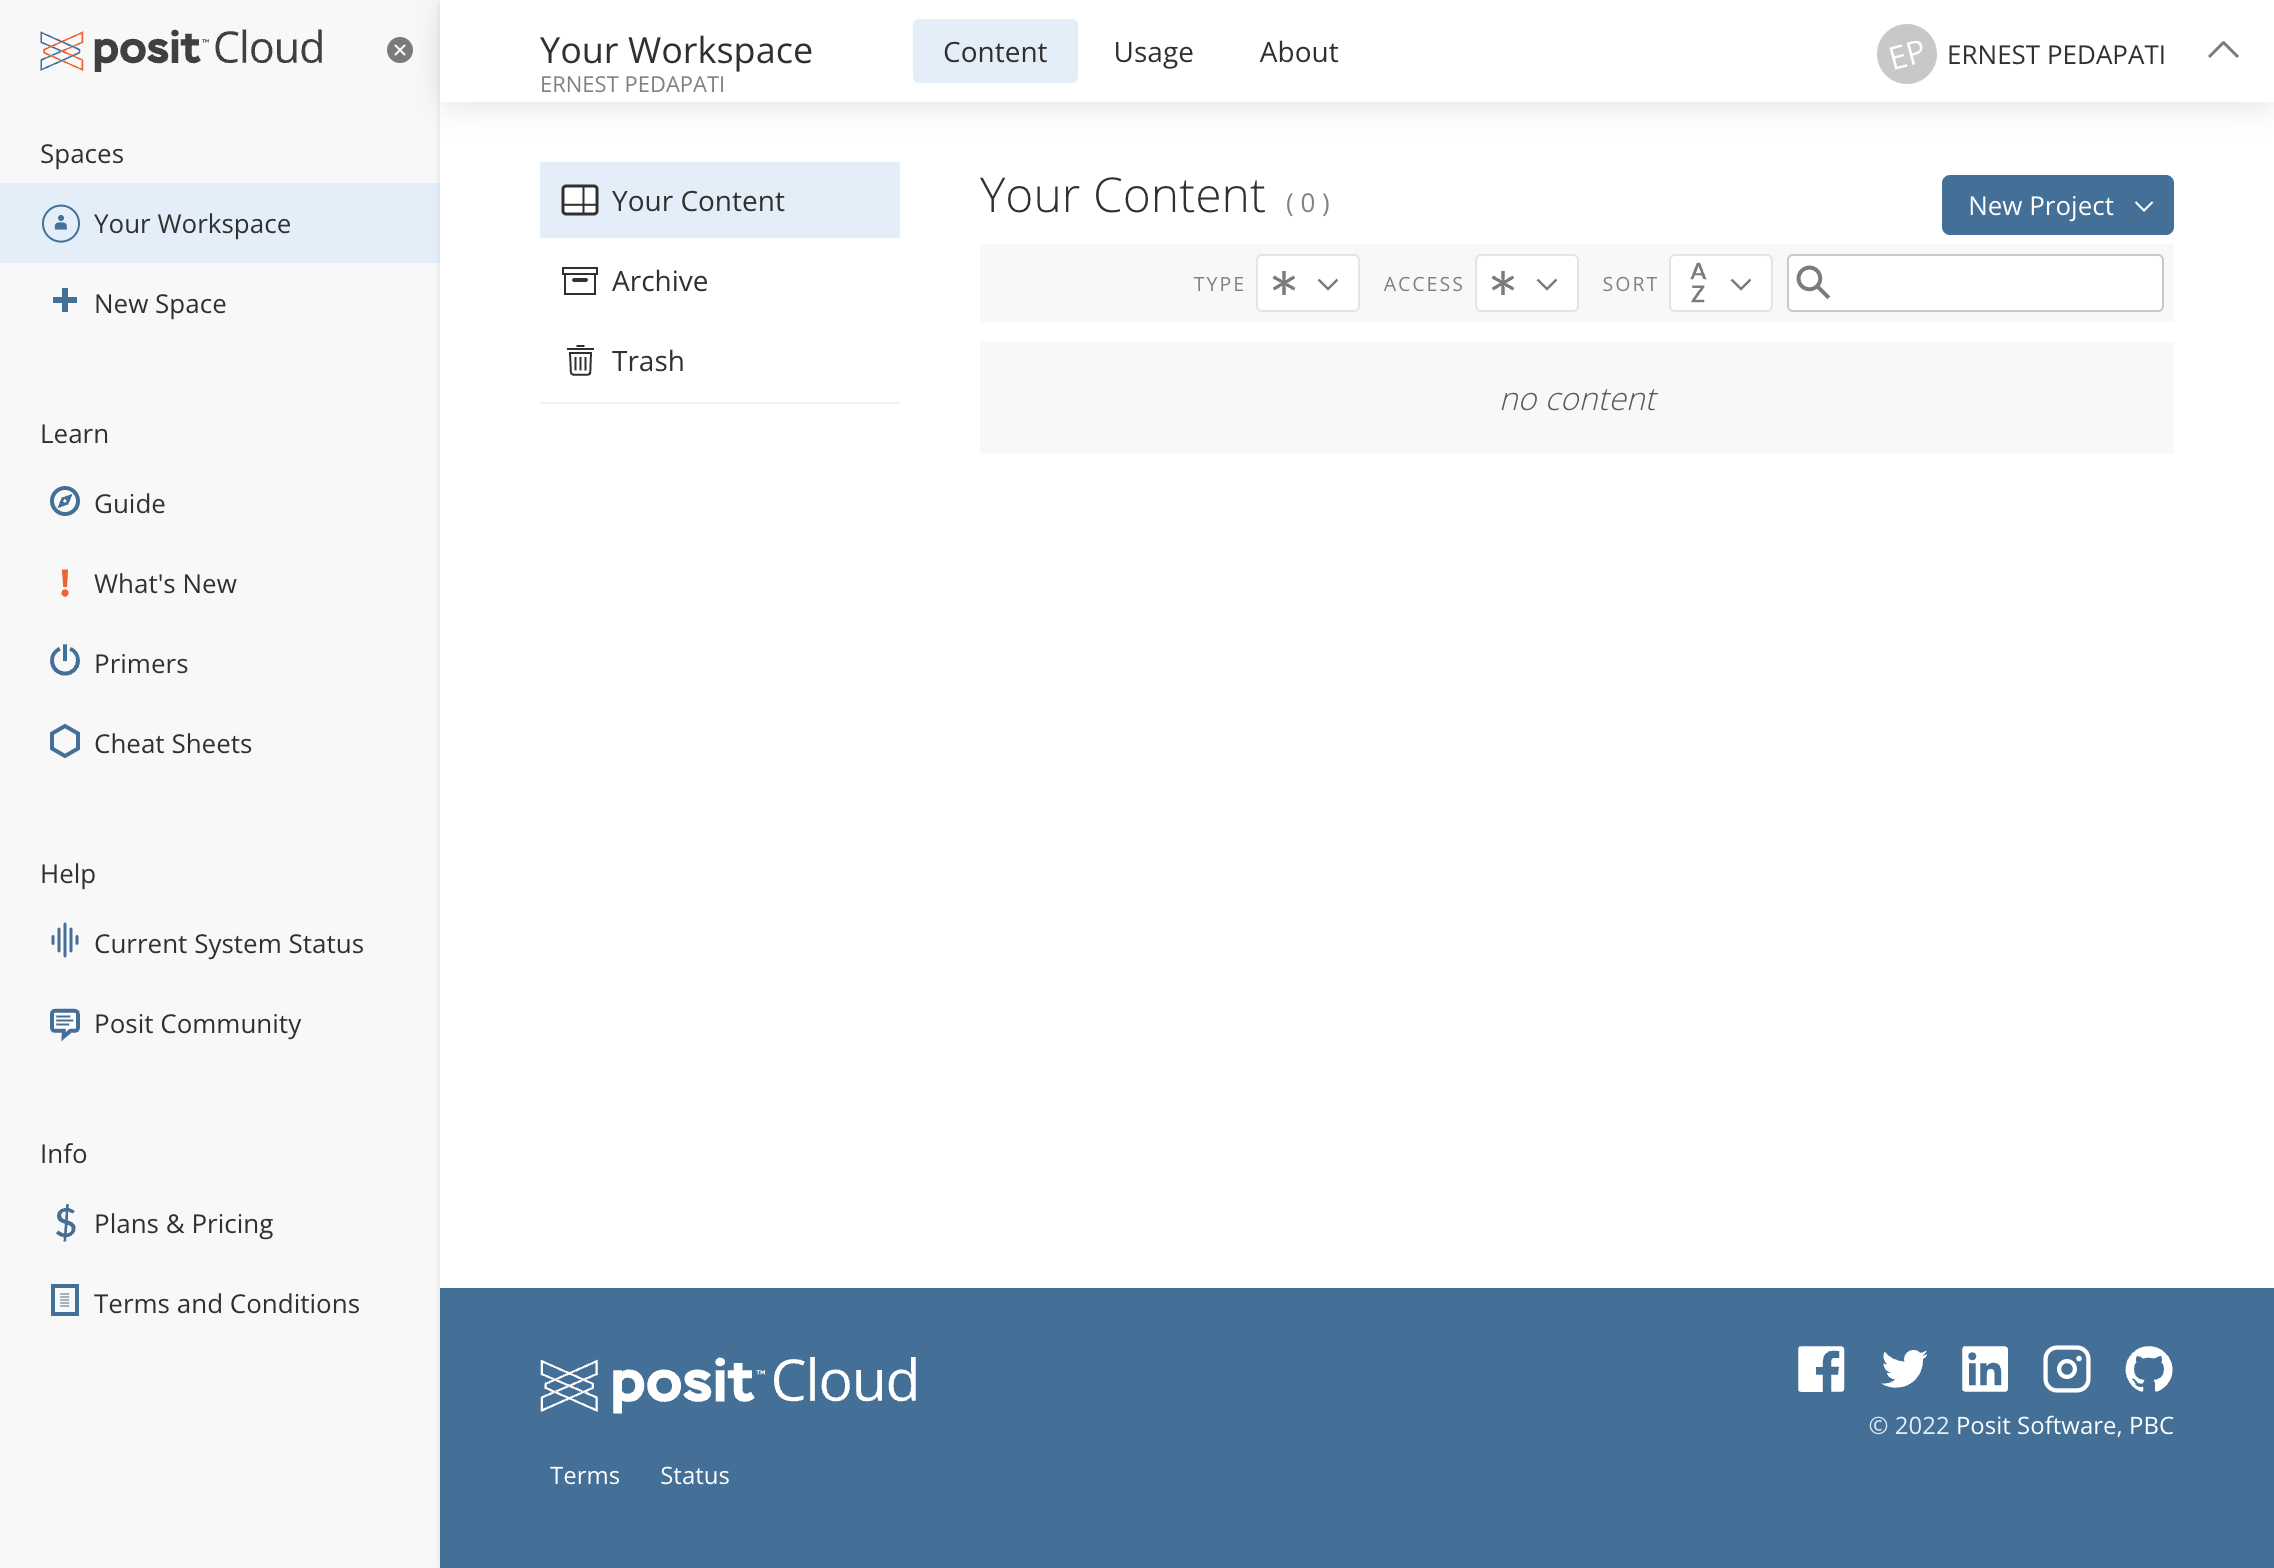
\includegraphics{./images/posit.cloud_login_code=sObwdDsWld0OQQ5q2vyhnQKQLbqk35.png}
  \end{quote}
\item
  \textbf{RStudio Cloud Interface}

  Now you're inside the RStudio interface, running within your web
  browser. On the left, you'll see the R console where you can enter R
  commands. The right panel contains tabs for plots, packages, help, and
  files. The top-left panel is for scripts or R Markdown files.

  \begin{quote}
  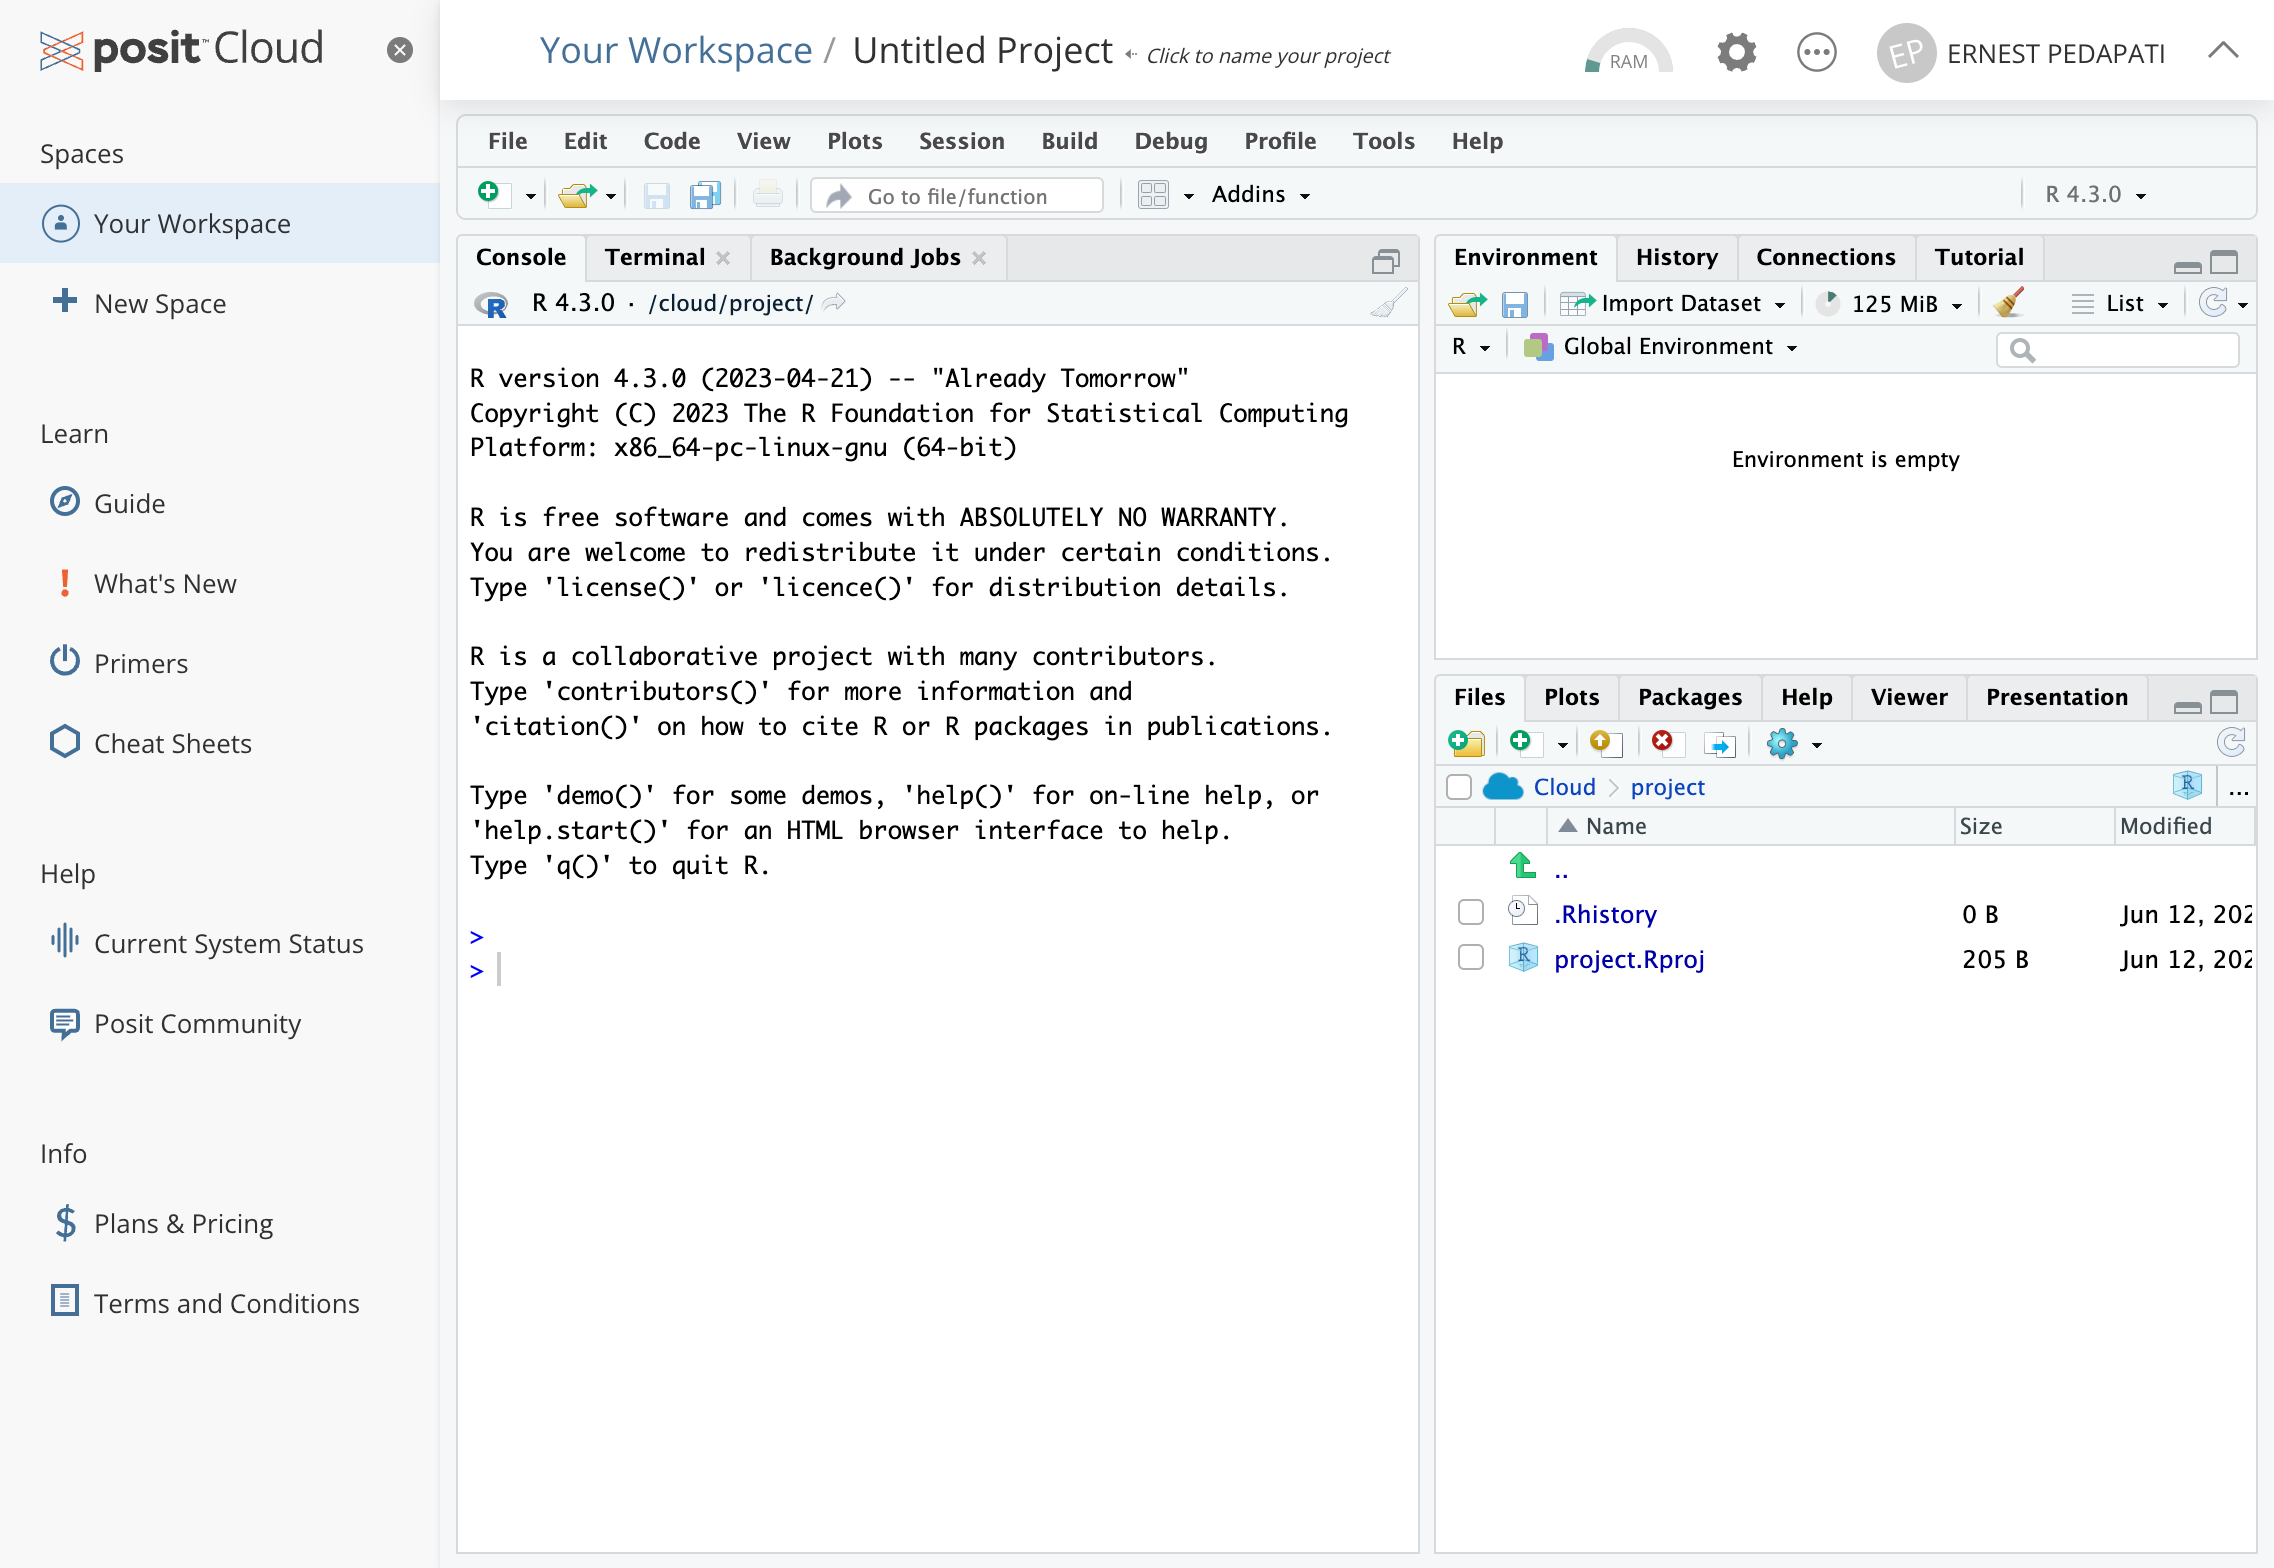
\includegraphics{./images/posit.cloud_login_code=sObwdDsWld0OQQ5q2vyhnQKQLbqk35 (1).png}
  \end{quote}
\item
  \textbf{Writing and Running R Code}

  To start coding, click on the ``File'' menu, then ``New File'', and
  then ``R Script''. An editor will open where you can write your R
  code. After writing your code, you can run it by clicking on the
  ``Run'' button, or by pressing Ctrl+Enter (Cmd+Enter on Mac).

  \begin{quote}
  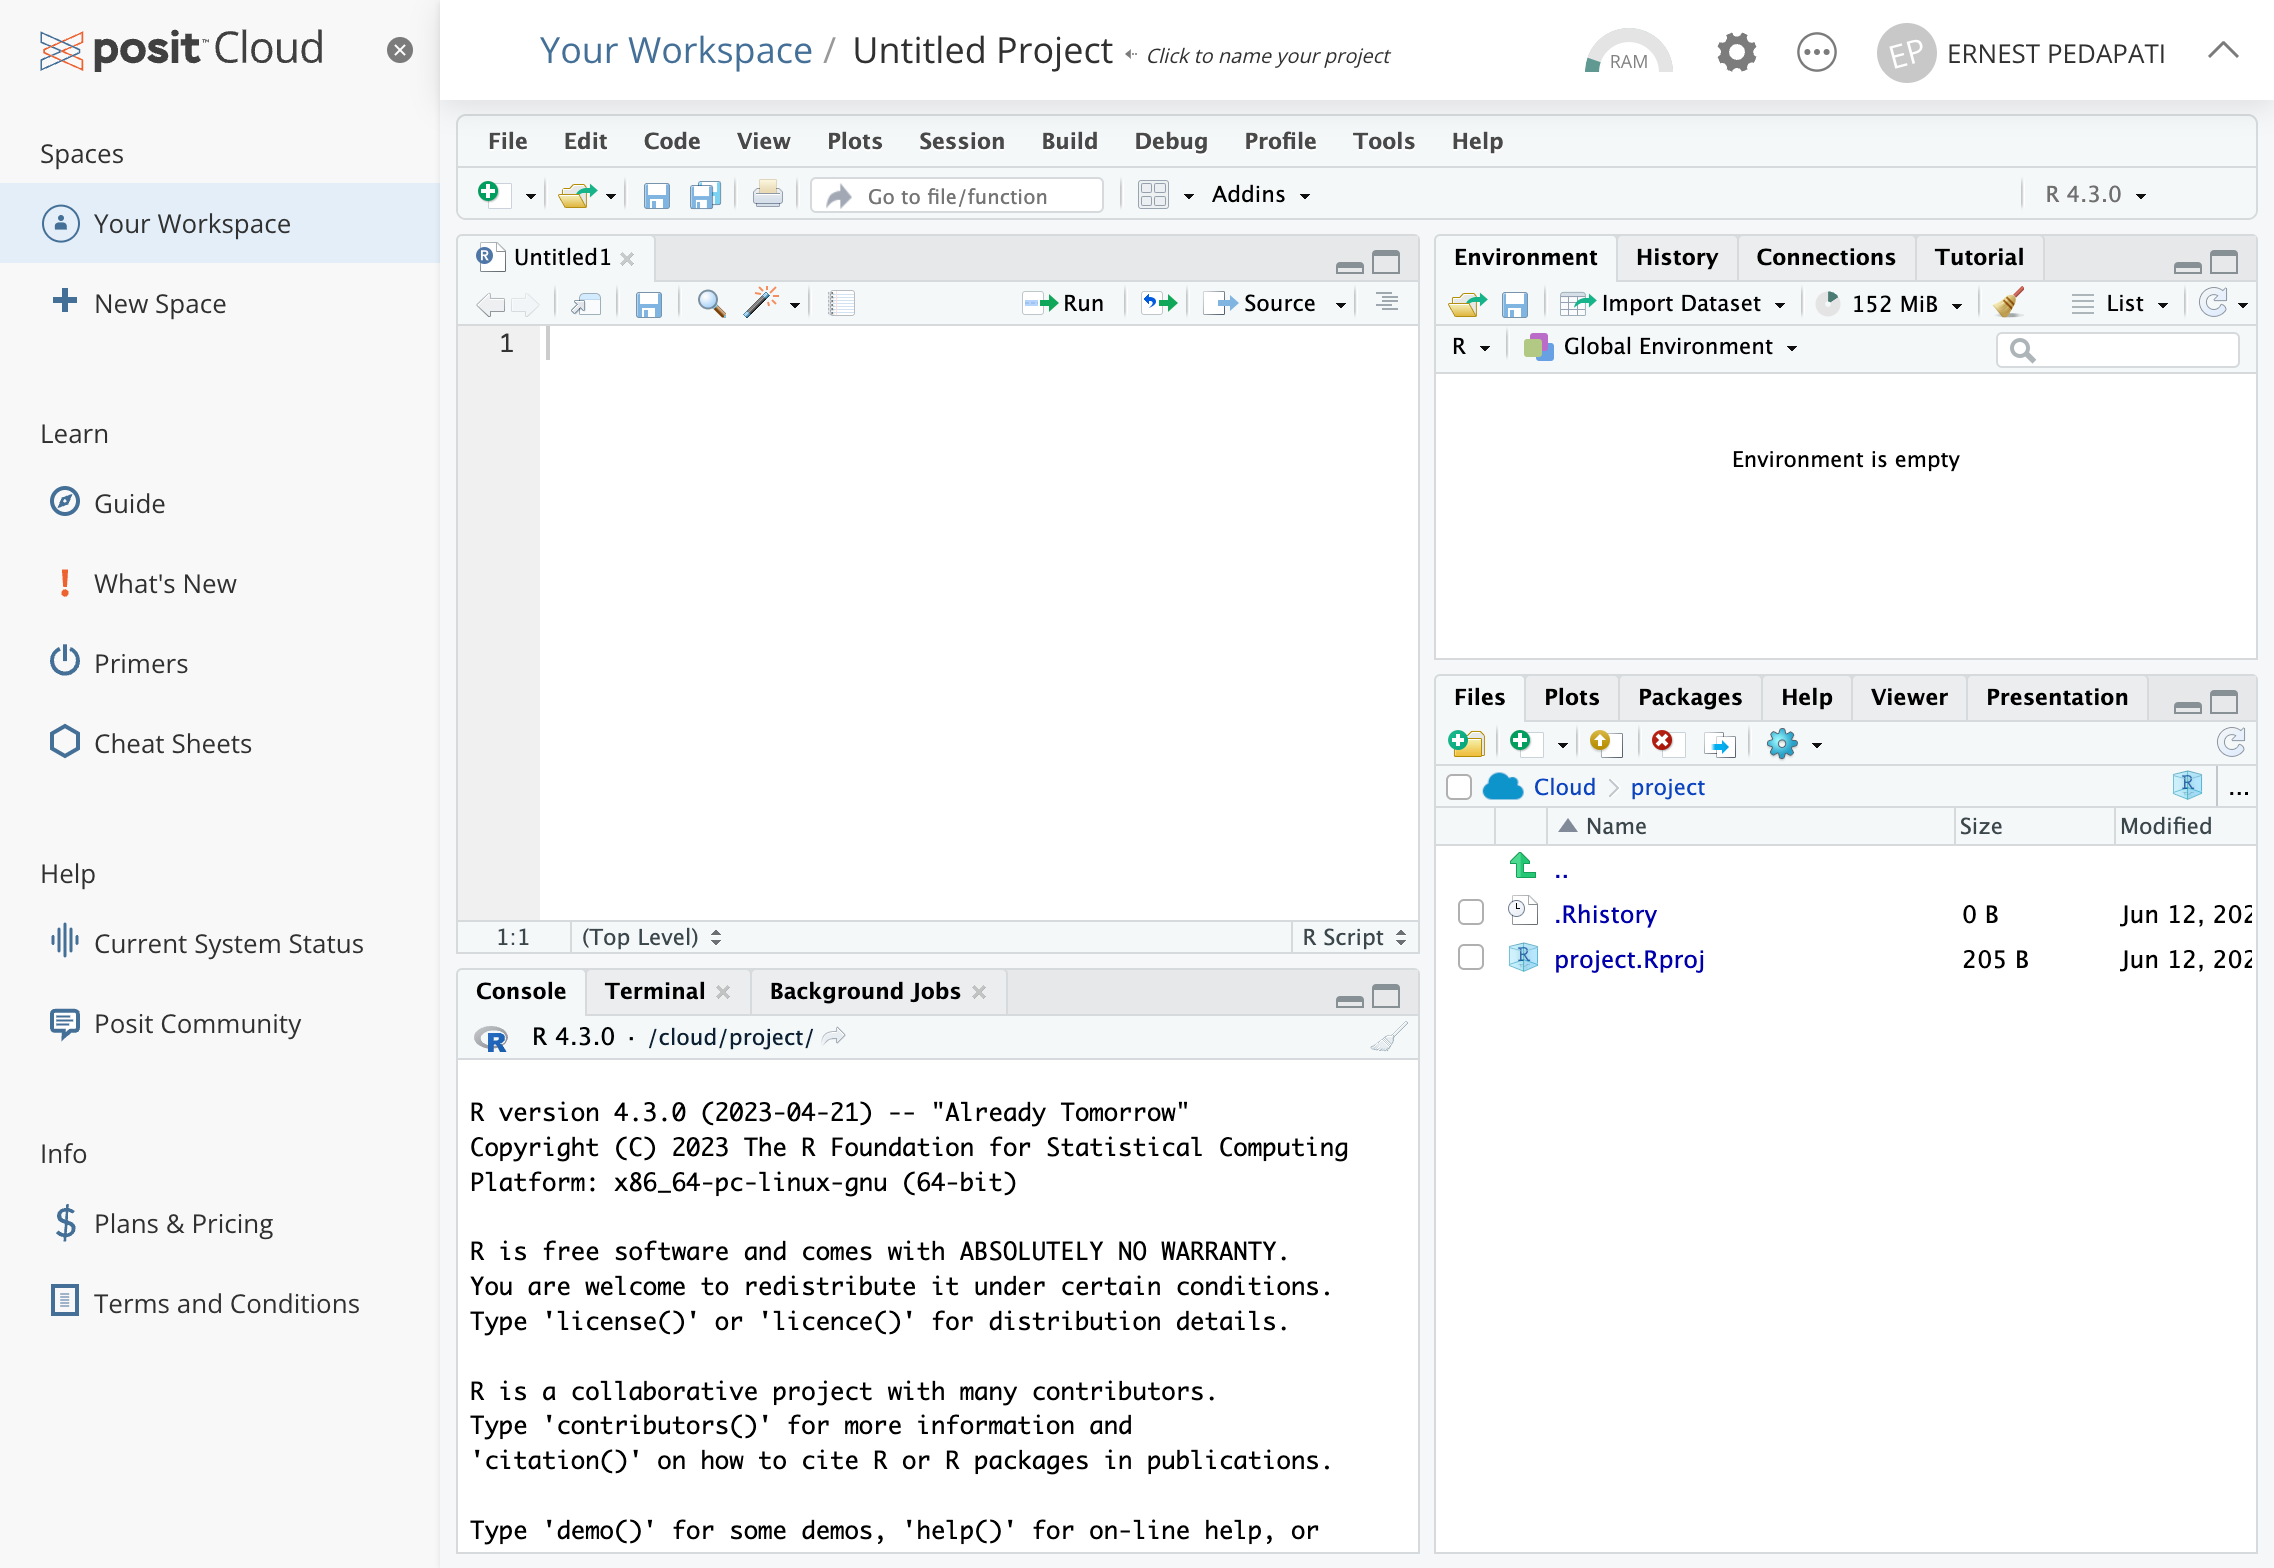
\includegraphics{./images/posit.cloud_login_code=sObwdDsWld0OQQ5q2vyhnQKQLbqk35 (3).png}
  \end{quote}
\item
  \textbf{Run some practice code}

  Let's test out your setup by printing ``Hello World!''. In your empty
  script type \texttt{print("Hellow\ World!")\textasciigrave{}} and
  click on the ``Run'' button.

  \begin{quote}
  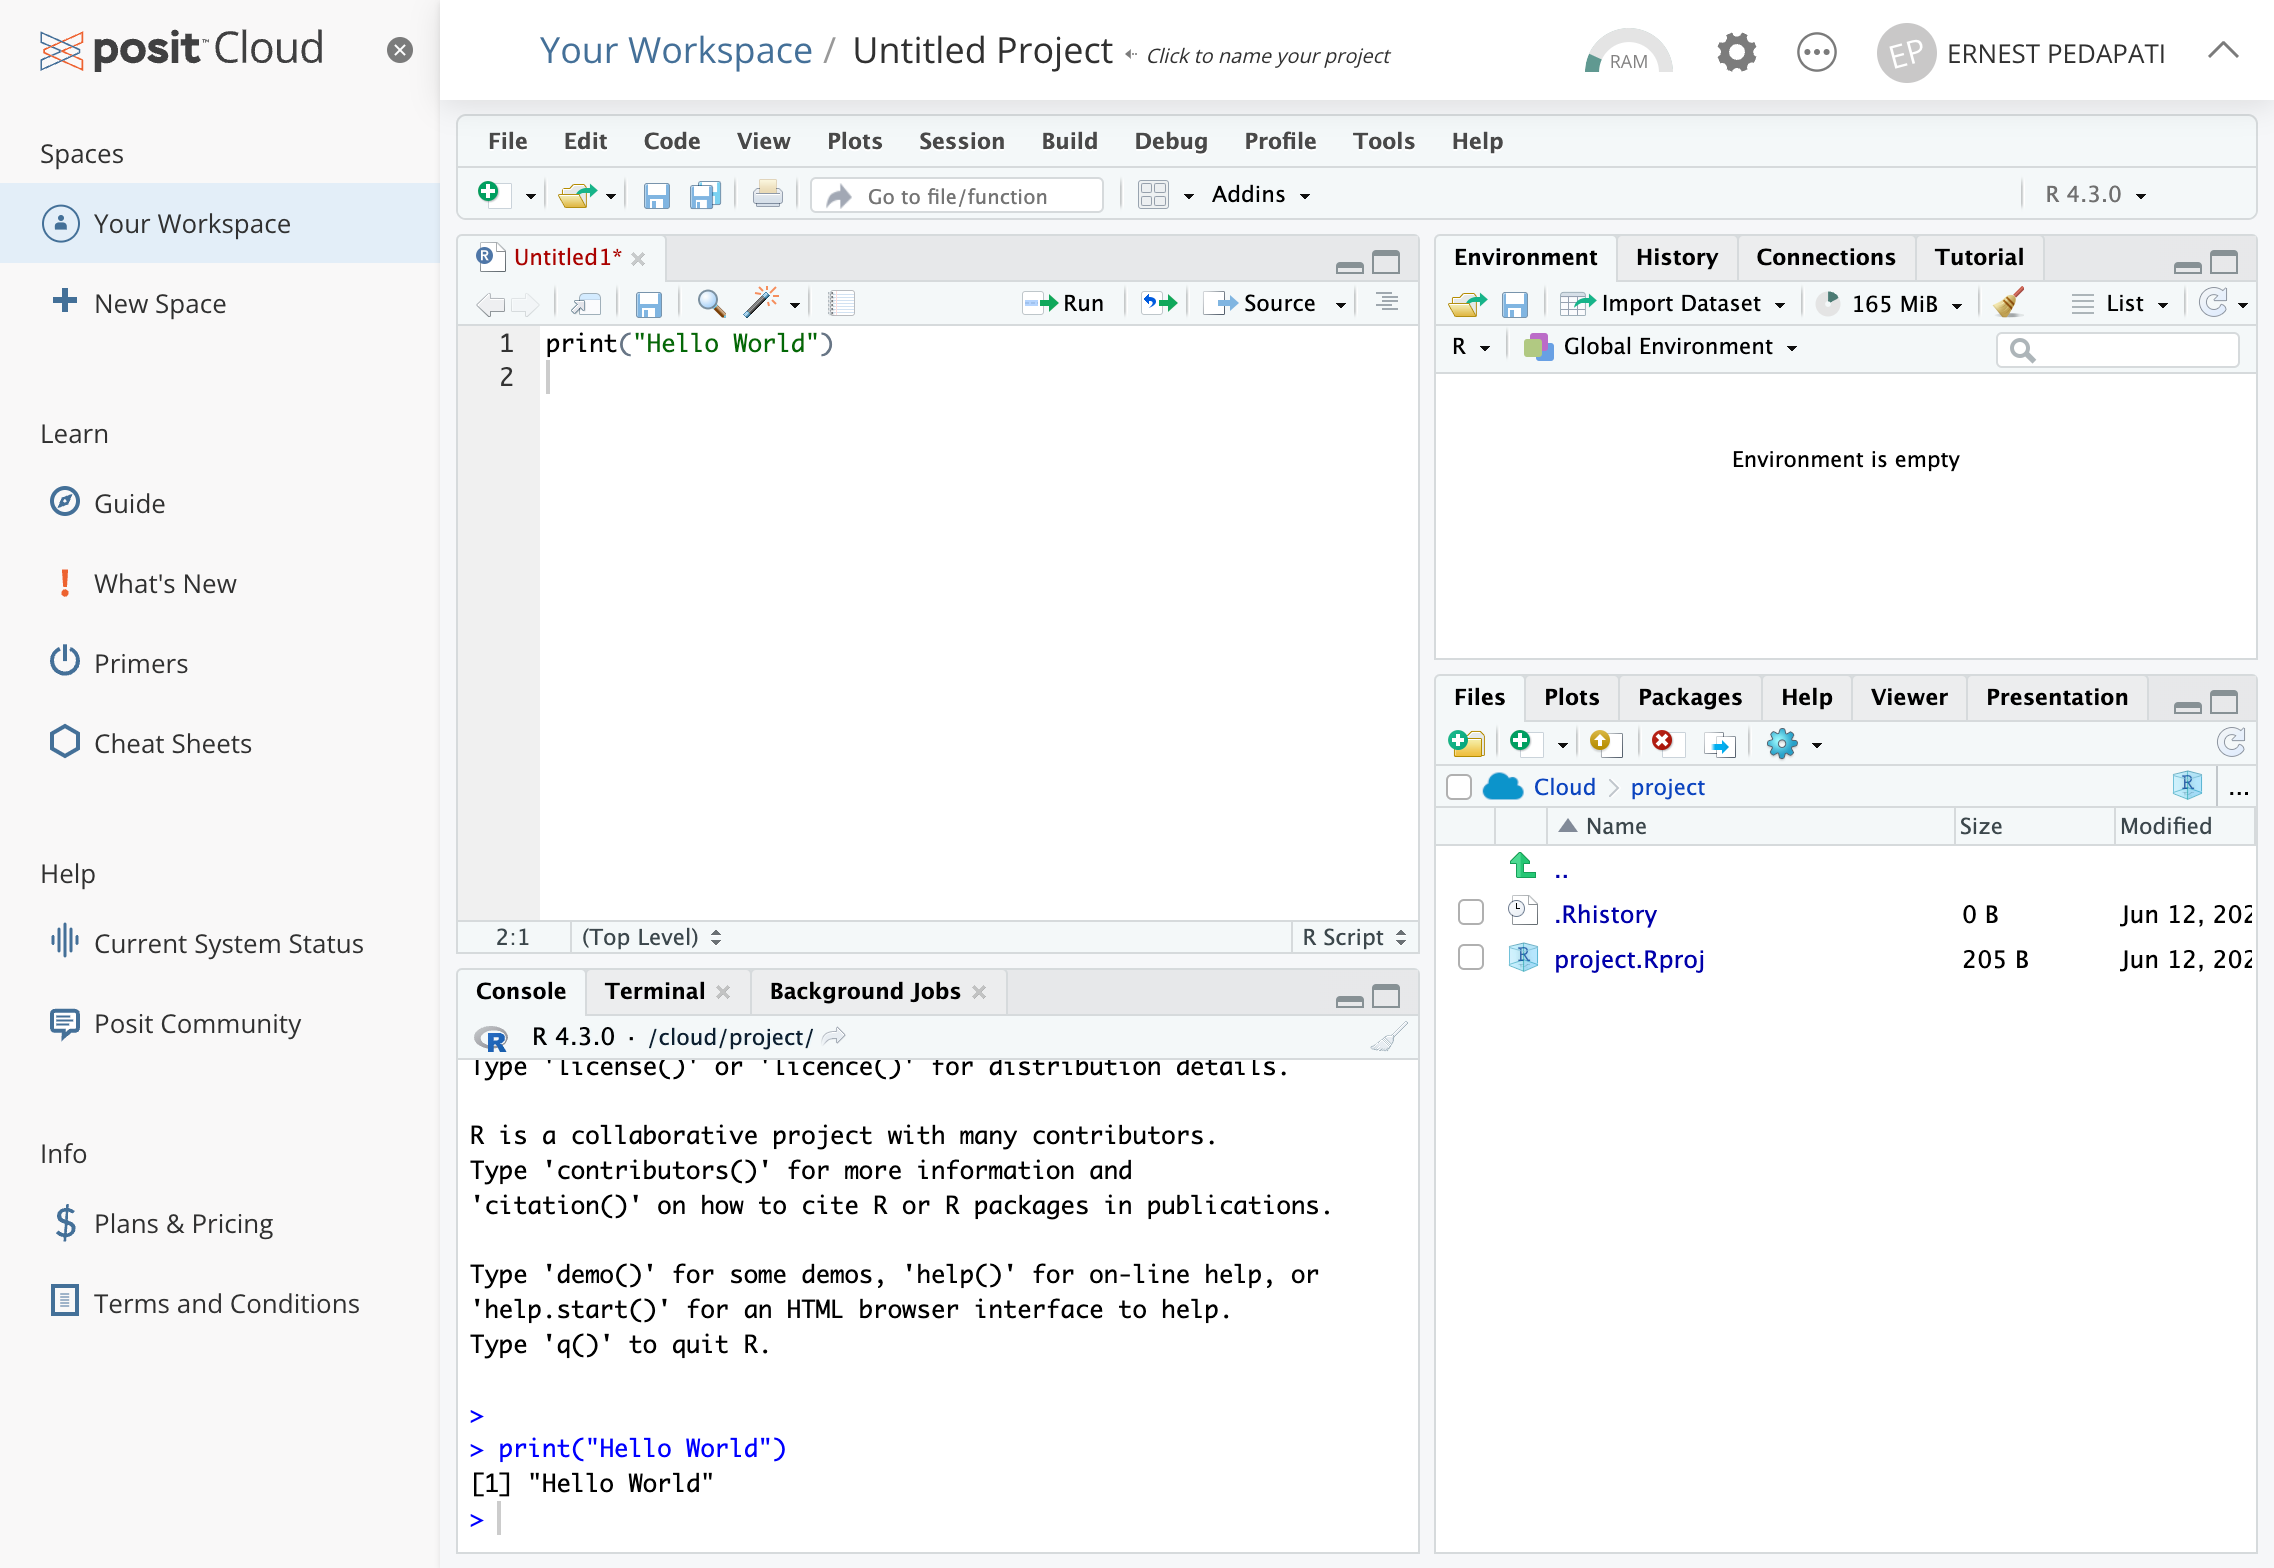
\includegraphics{./images/posit.cloud_login_code=sObwdDsWld0OQQ5q2vyhnQKQLbqk35 (2).png}
  \end{quote}
\item
  \textbf{Saving and Sharing Your Work}

  RStudio Cloud autosaves your work as you go, so you don't have to
  worry about losing your code. If you want to share your project, click
  on the ``Settings'' gear icon in the top-right corner of the project,
  and set ``Who can view this project'' to ``Everyone''. You can then
  share the URL of your project with others.

  \begin{quote}
  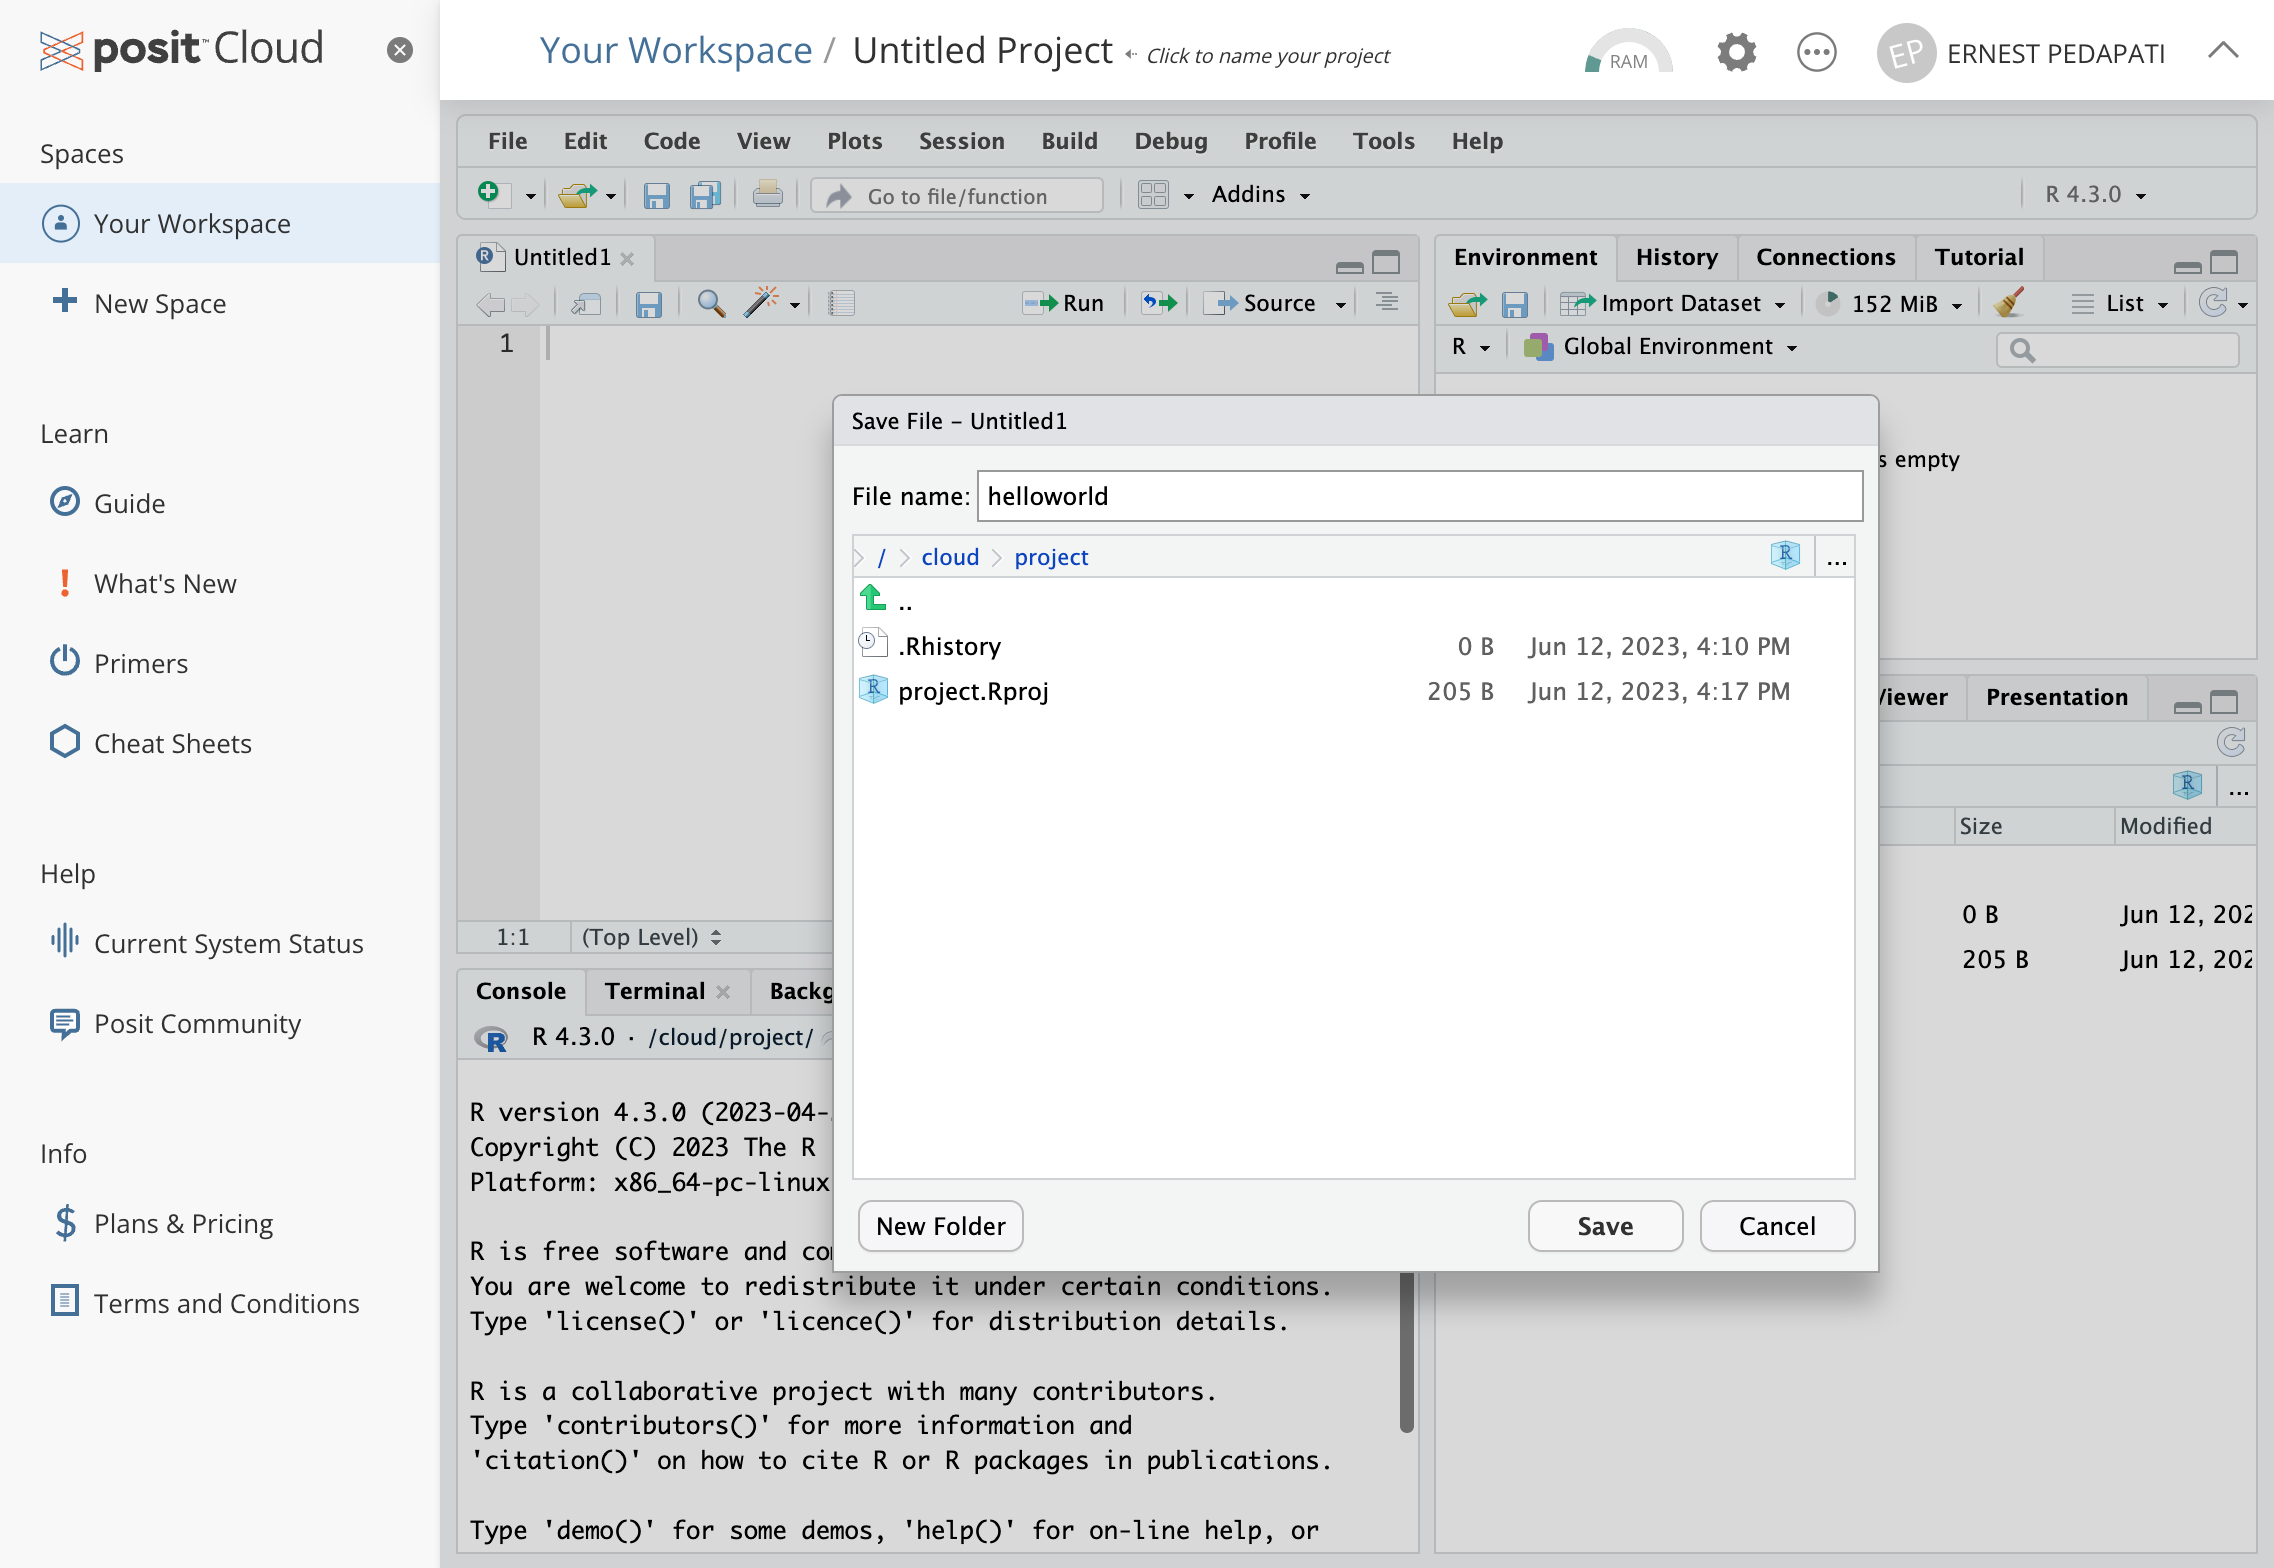
\includegraphics{./images/posit.cloud_login_code=sObwdDsWld0OQQ5q2vyhnQKQLbqk35 (4).png}
  \end{quote}
\end{enumerate}

Congratulations! You're now up and running with RStudio Cloud. You have
a versatile, powerful tool at your fingertips, ready to tackle your data
analysis needs.

\bookmarksetup{startatroot}

\hypertarget{getting-started-with-r}{%
\chapter{Getting Started with R}\label{getting-started-with-r}}

\hypertarget{chapter-highlights}{%
\section{Chapter highlights}\label{chapter-highlights}}

\begin{itemize}
\tightlist
\item
\end{itemize}

\hypertarget{introduction-to-the-data}{%
\section{Introduction to the data}\label{introduction-to-the-data}}

The \texttt{medicaldata} package is a collection of R datasets that are
relevant to medical research. It offers a robust collection of medical
datasets extracted from a wide range of study designs, including
randomized controlled trials, retrospective and prospective cohort
studies, and case-control studies. These datasets encompass a diverse
array of medical conditions and treatment approaches, providing rich
opportunities for learning, exploration, and analysis.

The package contains over 19 datasets, covering a wide range of medical
topics, including cancer, cardiovascular disease, diabetes, and mental
health. One of the datasets, `strep\_tb', for example, is drawn from the
groundbreaking 1948 trial of Streptomycin treatment for tuberculosis,
the first modern randomized, placebo-controlled clinical trial. The
datasets in the \texttt{medicaldata} package are all in a standard
format, which makes them easy to use with R.

\hypertarget{using-packages-in-r}{%
\section{Using packages in R}\label{using-packages-in-r}}

How do we get access to all of these interesting datasets?

The beauty of R lies in its simplicity and ease of access to a wealth of
data and tools. Unlike traditional methods where you might have to
navigate to a website, download files, and manually place them into
specific directories, R simplifies this process immensely. One of the
big advantages of R is that it provides the capability to access
numerous tools and datasets directly from the command line using a
single line of code.

\hypertarget{useful-analogy-packages-are-like-toolboxes}{%
\section{Useful Analogy: Packages are like
Toolboxes}\label{useful-analogy-packages-are-like-toolboxes}}

Think of R as large workshop with access to a main tool depot. with
access to lots of specialized toolkits. In this workshop you are
assigned a personal workbench. The toolboxes are designed and put
together by different craftsmen, making them unique in the tools they
contain. If you've identified a toolbox that you need for a specific
project, you first have to bring that toolbox into your workbench. In
fact, it would not be unusual to retrieve several toolkits depending on
needs of your project.

However, just lugging the toolboxes to your workbench doesn't
necessarily mean you can immediately use the tools they contains. If you
want access to all your screwdrivers at once, you will need open a
specialized screwdriver toolkit. On the other hand, you might only want
a single screwdriver from a special toolkit. this is more than just
keeping your workbench tidy, you also don't want to have duplicates of
similar tools around which may lead to confusion.

\hypertarget{breaking-down-the-workshop-analogy}{%
\section{Breaking down the workshop
analogy}\label{breaking-down-the-workshop-analogy}}

Let's connect this analogy with learning R

\begin{itemize}
\item
  The workshop represents R and RStudio
\item
  The personal workbench is your R project
\item
  The toolboxes are R packages
\item
  The tool depot is the Comprehensive R Archive Network (CRAN) package
  repository (more on this later!)
\item
  Lugging the toolkit to your workbench is analogous to installing the
  package
\item
  Opening the entire toolkit is adding it to your active R libraries
\item
  Selecting a single tool from a toolkit is the same as using the
  \texttt{::} operator on a package.
\end{itemize}

\hypertarget{software-repositories-in-r}{%
\section{Software repositories in R}\label{software-repositories-in-r}}

\hypertarget{cran-httpscran.r-project.org}{%
\subsection{\texorpdfstring{CRAN
(\url{https://cran.r-project.org/})}{CRAN (https://cran.r-project.org/)}}\label{cran-httpscran.r-project.org}}

The CRAN repository where officially approved and tested packages are
stored.These packages are well-documented, reliable, and updated
regularly. So, if you need a tool for a common task, you're likely to
find a toolbox containing it in the CRAN repository.

\hypertarget{development-repositories}{%
\subsection{Development repositories}\label{development-repositories}}

Places like Github and other code repositories offer exciting,
cutting-edge tools that may not have made their way to the main CRAN
depot yet. While the tools from these workshops can be highly useful,
they also come with a word of caution as they may not be as thoroughly
tested and documented as those in the CRAN depot. You may also you need
to use the latest advancements with well-known packages that have not
been updated on CRAN yet.

\hypertarget{walkthrough}{%
\section{Walkthrough}\label{walkthrough}}

Let's walk through loading the \texttt{medicaldata} package which will
provide the datasets we will use thoughout the rest of book.

\hypertarget{setting-the-stage}{%
\subsection{Setting the stage}\label{setting-the-stage}}

\begin{enumerate}
\def\labelenumi{\arabic{enumi}.}
\tightlist
\item
  First create a new R project in R Cloud
\end{enumerate}

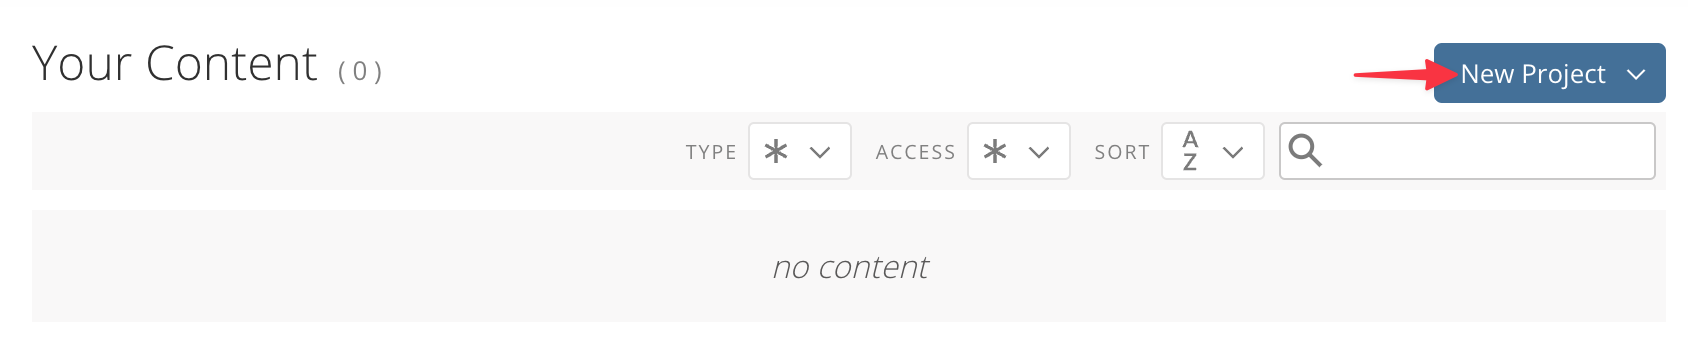
\includegraphics{./images/posit.cloud_login_code=RjaPWEO8K1VLgeNKrf5fPzXTp4ezfa (1)-01.png}

\begin{enumerate}
\def\labelenumi{\arabic{enumi}.}
\setcounter{enumi}{1}
\tightlist
\item
  Create a new empty R script
\end{enumerate}

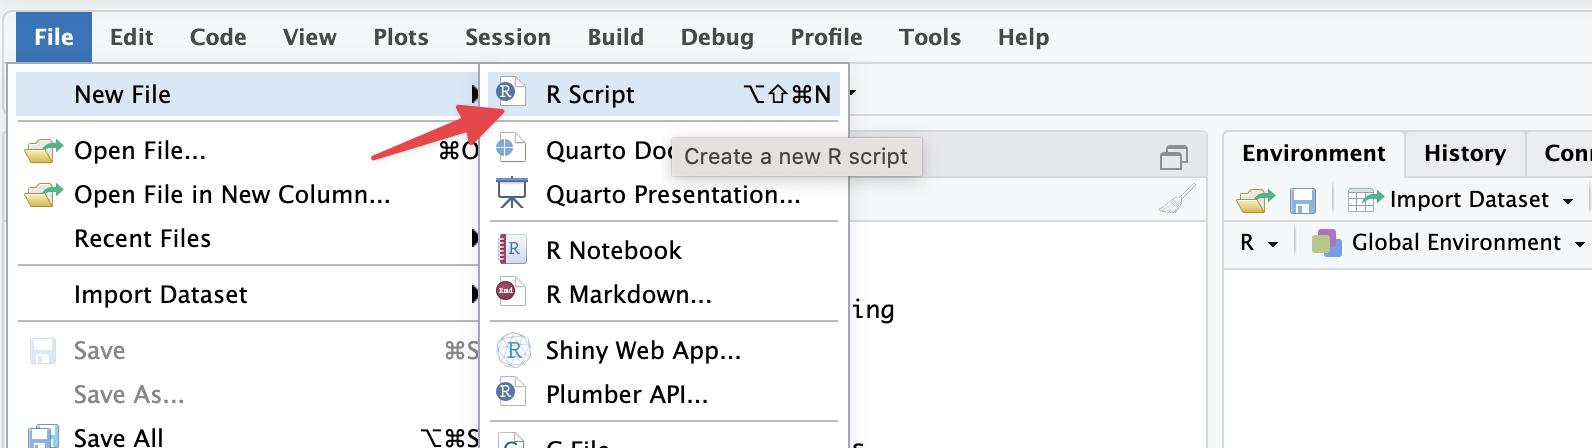
\includegraphics{./images/CleanShot 2023-06-12 at 22.18.53@2x.png}

\begin{enumerate}
\def\labelenumi{\arabic{enumi}.}
\setcounter{enumi}{2}
\item
  Save the File as chapter1.R

  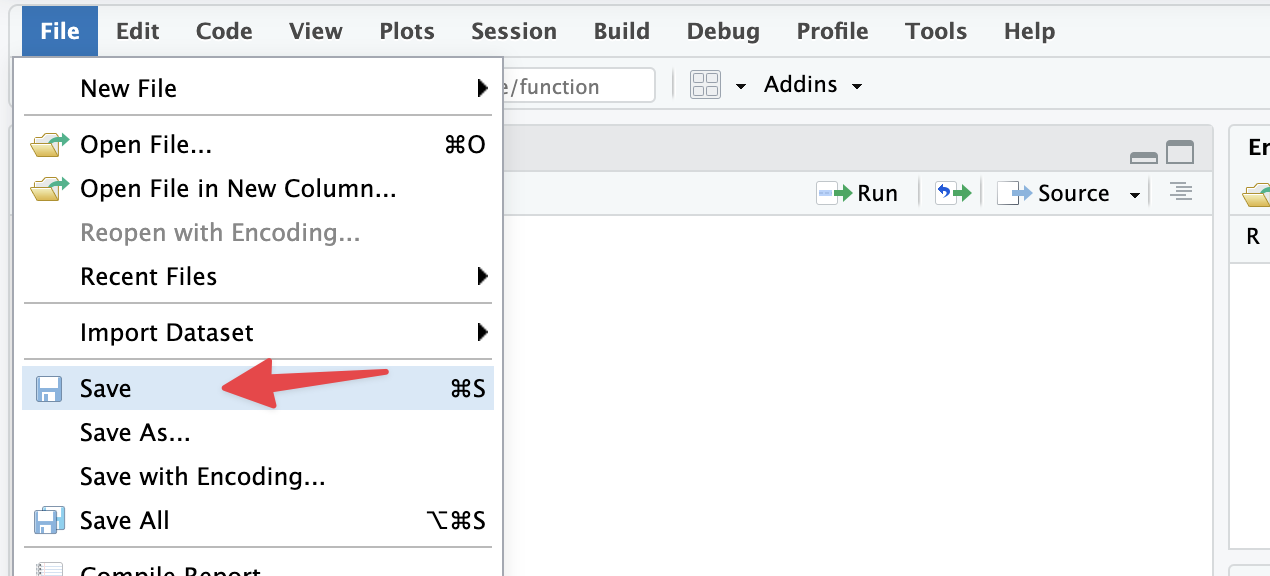
\includegraphics{./images/CleanShot 2023-06-12 at 22.21.34@2x.png}
\item
  Type the following into your blank script:
\end{enumerate}

\begin{Shaded}
\begin{Highlighting}[]
\CommentTok{\# Install the R package medicaldata}
\FunctionTok{install.packages}\NormalTok{(}\StringTok{"medicaldata"}\NormalTok{)}

\CommentTok{\# Load package into active library}
\FunctionTok{library}\NormalTok{(medicaldata)}
\end{Highlighting}
\end{Shaded}

\begin{enumerate}
\def\labelenumi{\arabic{enumi}.}
\setcounter{enumi}{4}
\tightlist
\item
  Access the \texttt{Code} menu and select \texttt{Run\ All}
\end{enumerate}

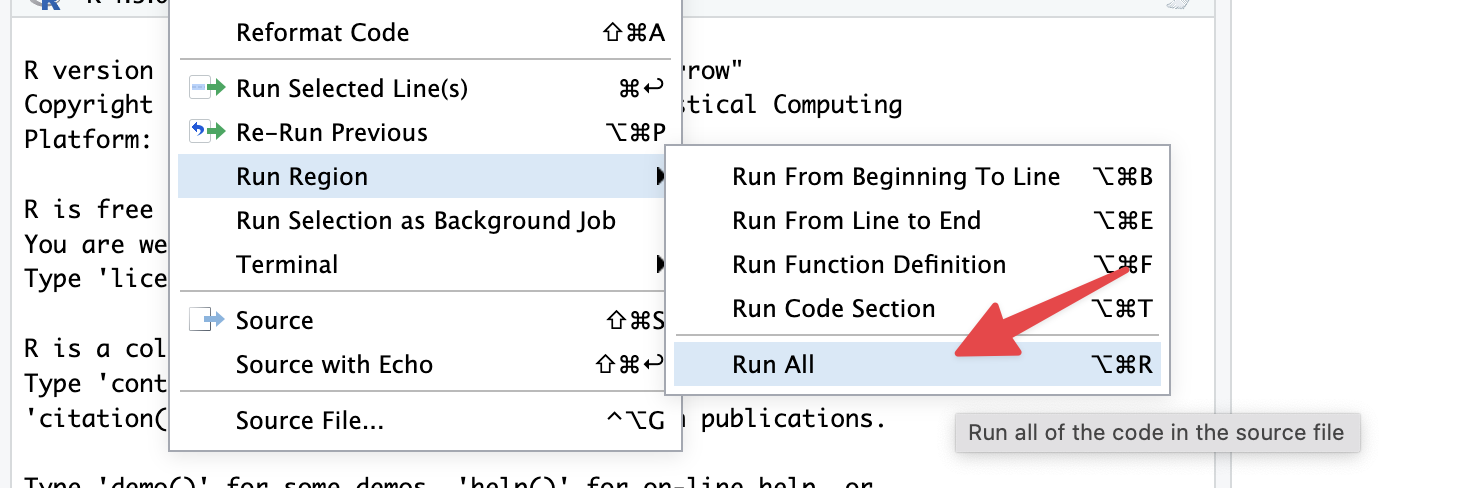
\includegraphics{./images/CleanShot 2023-06-12 at 22.26.59@2x.png}

\begin{enumerate}
\def\labelenumi{\arabic{enumi}.}
\setcounter{enumi}{5}
\tightlist
\item
  Examine the output in the console window.
\end{enumerate}

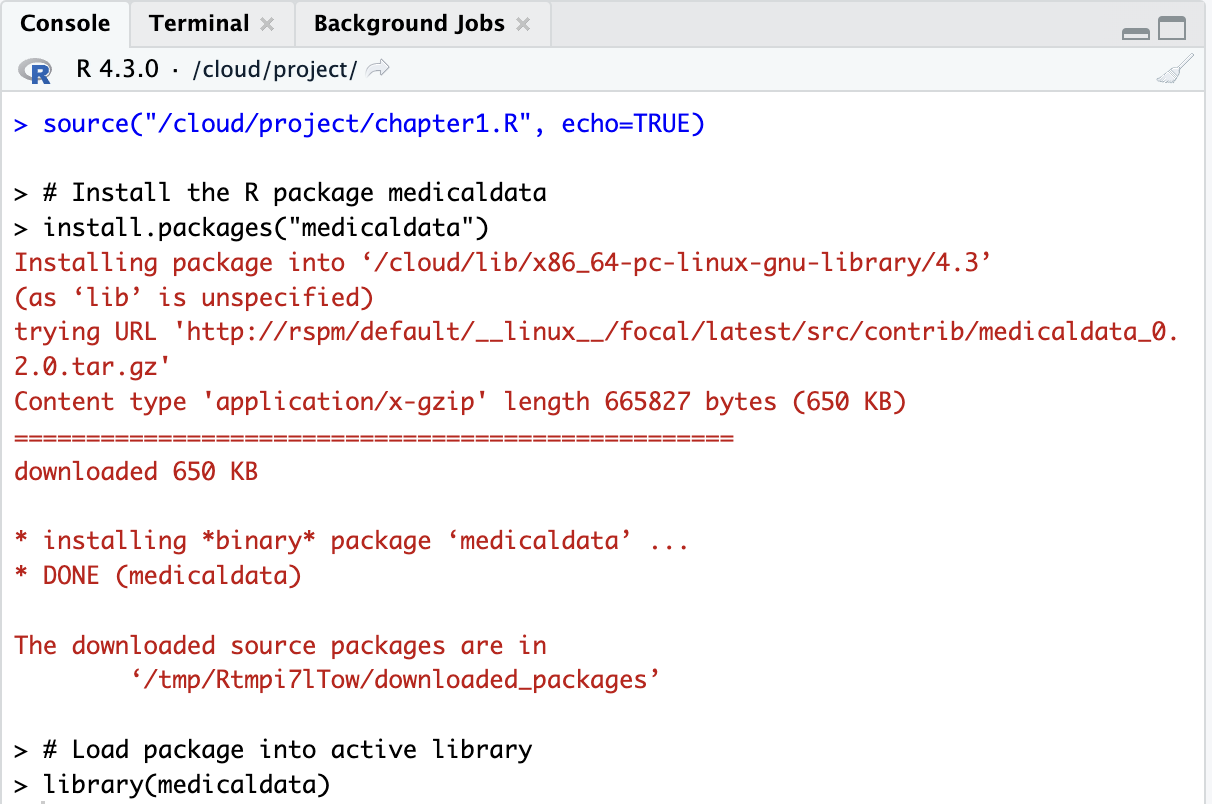
\includegraphics{./images/CleanShot 2023-06-12 at 22.29.32@2x.png}

\hypertarget{reviewing-the-code}{%
\section{Reviewing the Code}\label{reviewing-the-code}}

Diving into the code we've written, several key points need to be
highlighted.

\begin{itemize}
\item
  Code isn't like regular writing. Forget paragraphs; each command you
  write stands alone on its own line.
\item
  The pound symbol \# leads us to the next key point. Placing this at
  the start of a line tells R to gloss over this part when executing
  code. This is what we call a comment and it's a handy way to leave
  notes for yourself and others.
\item
  The third point concerns functions, such as
  \texttt{install.packages()} and \texttt{library()}. Consider functions
  as time-saving shortcuts for complicated operations. They take inputs
  and give outputs.
\item
  When you see parentheses associated with a term, think function.
  Whatever goes inside these parentheses are known as input parameters
  to the function.
\item
  Look closely at the use of quotes around \texttt{medicaldata} in the
  \texttt{install.packages} line, but their absence in the
  \texttt{library} line. In R, quotes aren't just punctuation, they
  serve a specific function which we'll delve deeper into later.
\end{itemize}

\hypertarget{examining-the-output}{%
\section{Examining the output}\label{examining-the-output}}

Our first interactive coding command produced some interesting output in
the R console. Let's take a moment to discuss the R console and
understand what it just told us.

The R console is akin to a live conversation with R. When you type a
command and hit enter, R listens, processes the request, and then speaks
back to you. This ``speech'' is the output you see on your screen. Let's
look at the output from our script.

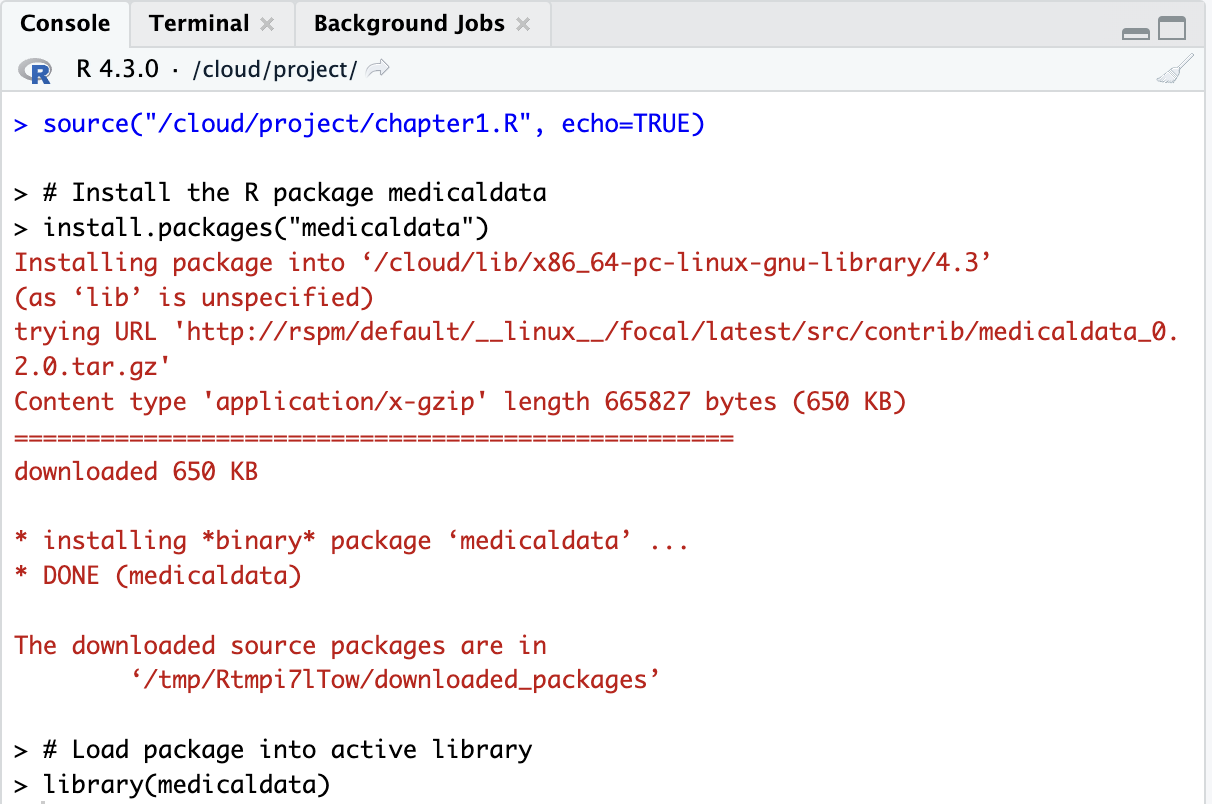
\includegraphics{./images/CleanShot 2023-06-12 at 22.29.32@2x-01.png}

Now, back to the output of our first command,
\textbf{\texttt{install.packages("medicaldata")}}. This command tells R
to install the ``medicaldata'' package, a collection of ready-made
functions and data. R takes this command, connects to a server, and
starts to download the package. It provides us with live updates,
telling us how large the package is (650 KB), and its download status.

The next few lines,
\textbf{\texttt{*\ installing\ *binary*\ package\ ‘medicaldata’\ ...}}
and \textbf{\texttt{*\ DONE\ (medicaldata)}}, tell us that R has
successfully installed the package.

The last line of the output,
\textbf{\texttt{‘/tmp/Rtmpi7lTow/downloaded\_packages’}}, is R's way of
saying ``If you need the downloaded files, here's where I've stored
them''.

Once the installation is complete, we run
\textbf{\texttt{library(medicaldata)}}. This command tells R to open the
toolbox of \texttt{medicaldata} and make its tools available for use.
There's no output after this command, which usually indicates that the
command has run successfully and the package is ready to use.

\hypertarget{checking-the-results-of-our-work}{%
\section{Checking the results of our
work}\label{checking-the-results-of-our-work}}

Installing packages is a fundamental aspect of using R. In the next few
chapters we will learn more about the language of R to manipulate and
process data, but for now let's see the fruit of our labor.

Most R packages have excellent documentation. The medicaldata package is
no exception. The guide to the datasets in the package can be found at
this link: \url{https://higgi13425.github.io/medicaldata/}.

Let's use the instructions from the package author to view the different
datasets we now have installed by typing into the console:

\begin{Shaded}
\begin{Highlighting}[]
\FunctionTok{data}\NormalTok{(}\AttributeTok{package =} \StringTok{"medicaldata"}\NormalTok{)}
\end{Highlighting}
\end{Shaded}

Once you execute this command, R will display an interactive window
showing you all the datasets available in the ``medicaldata'' package.
Each dataset is listed with a brief description of the kind of data it
contains, which can be very useful when deciding which dataset to use
for a particular analysis.

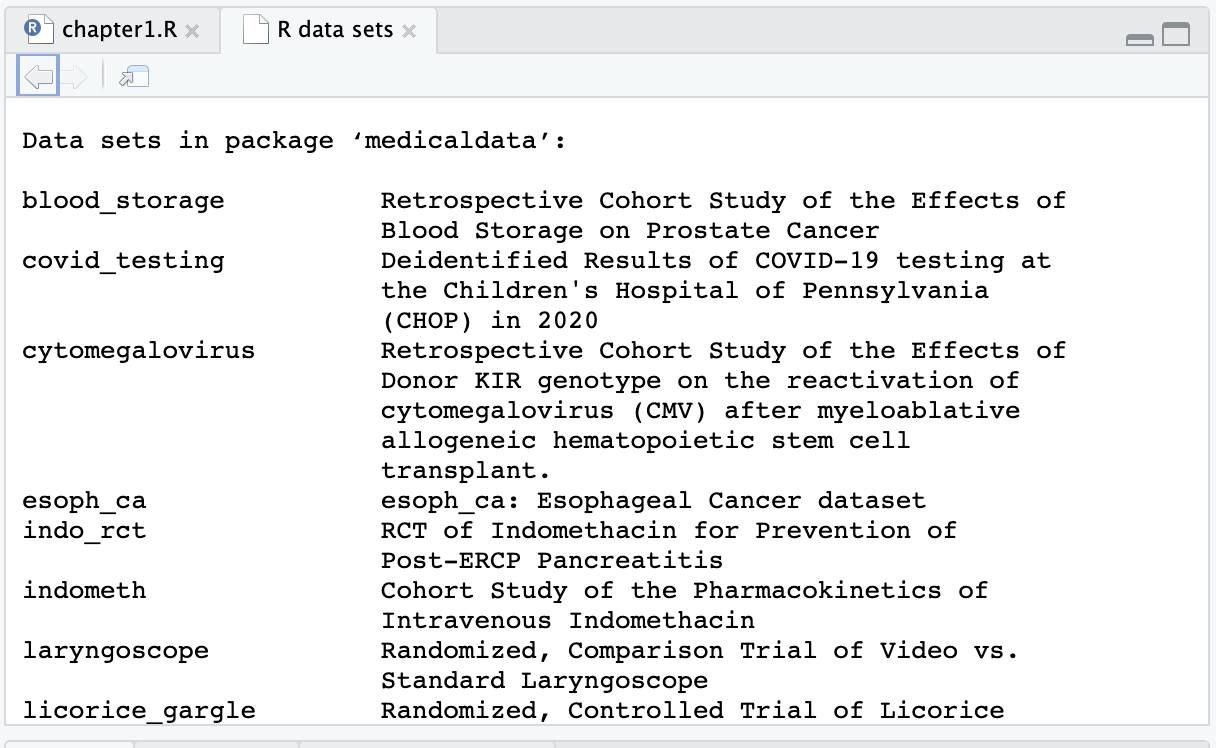
\includegraphics{./images/CleanShot 2023-06-12 at 23.00.17@2x.png}

\hypertarget{entering-data-within-a-script-versus-the-console}{%
\section{Entering data within a script versus the
console}\label{entering-data-within-a-script-versus-the-console}}

When you're working with R, you have two main places where you can enter
your data or commands: the script editor and the console.

The script editor is your workspace for crafting R scripts. This is
where you write your lines of code, organize your thoughts, define
functions, and generally create your R programs. Anything you write in
the script editor is saved and can be run as many times as you want,
making it ideal for larger, more complex analyses.

On the other hand, the console is the live interaction space where R
executes commands and displays results. Anything you type directly into
the console is run immediately, but it's not saved once you close your R
session. It's a great place for quick calculations, testing small bits
of code, or inspecting data.

In essence, the script editor is your drafting table where you design
and plan, and the console is more like a chat where you can immediately
execute and see your plans come to life. As you continue to work with R,
you'll become more comfortable determining when to use each for
different tasks.

Indeed, certain commands are best suited for direct execution in the
console, especially those that serve to inspect data or check a
package's contents. The command to view the datasets within the
\textbf{\texttt{medicaldata}} package is a good example of this. It's a
`single-use' operation that doesn't necessarily form part of the core
workflow in your script, but rather provides you with valuable
contextual information.

\hypertarget{chapter-summary}{%
\section{Chapter Summary}\label{chapter-summary}}

In this chapter, we introduced the basics of using R, with a specific
focus on accessing and utilizing packages from CRAN. We introduced the
concept of functions, explained the role of comments, and highlighted
the differences between writing code in a script versus executing
commands in the console. Through the installation and exploration of the
`medicaldata' package, we demonstrated the ease and power of working
with packages in R. This foundational knowledge will serve as a solid
base as we delve deeper into R programming in subsequent chapters.

\bookmarksetup{startatroot}

\hypertarget{summary}{%
\chapter{Summary}\label{summary}}

This book is designed as a guide, a companion on your journey to
mastering R, but it's not just another instruction manual. As a fellow
physician who discovered the power of R after my residency, I've
encountered and navigated the same challenges you're likely to face.
This book synthesizes those experiences into a streamlined learning path
that addresses our unique needs and use-cases in the medical field. It
is a comprehensive roadmap, crafted to transform you from an R novice to
a confident user, capable of leveraging this powerful tool to improve
your research, data analysis, and overall work.

Our goal is not to become software engineers or statisticians, but
rather to harness the potential of R to make our tasks more efficient
and our decisions more data-driven. To this end, this book covers the
essentials of R programming, data manipulation, statistical analysis,
and data visualization. Moreover, the lessons are grounded in
real-world, relatable examples, including using medical datasets, making
the learning experience engaging and intuitive. By the end of this book,
you will have gained a robust understanding of R, its application in
healthcare, and most importantly, the confidence to explore further and
ask the right questions of your data.

\bookmarksetup{startatroot}

\hypertarget{references}{%
\chapter*{References}\label{references}}
\addcontentsline{toc}{chapter}{References}

\markboth{References}{References}

\hypertarget{refs}{}
\begin{CSLReferences}{0}{0}
\end{CSLReferences}



\end{document}
